
\documentclass{article} % For LaTeX2e
\usepackage{iclr2021_conference,times}

% Optional math commands from https://github.com/goodfeli/dlbook_notation.
%%%%% NEW MATH DEFINITIONS %%%%%

\usepackage{amsmath,amsfonts,bm}

% Mark sections of captions for referring to divisions of figures
\newcommand{\figleft}{{\em (Left)}}
\newcommand{\figcenter}{{\em (Center)}}
\newcommand{\figright}{{\em (Right)}}
\newcommand{\figtop}{{\em (Top)}}
\newcommand{\figbottom}{{\em (Bottom)}}
\newcommand{\captiona}{{\em (a)}}
\newcommand{\captionb}{{\em (b)}}
\newcommand{\captionc}{{\em (c)}}
\newcommand{\captiond}{{\em (d)}}

% Highlight a newly defined term
\newcommand{\newterm}[1]{{\bf #1}}


% Figure reference, lower-case.
\def\figref#1{figure~\ref{#1}}
% Figure reference, capital. For start of sentence
\def\Figref#1{Figure~\ref{#1}}
\def\twofigref#1#2{figures \ref{#1} and \ref{#2}}
\def\quadfigref#1#2#3#4{figures \ref{#1}, \ref{#2}, \ref{#3} and \ref{#4}}
% Section reference, lower-case.
\def\secref#1{section~\ref{#1}}
% Section reference, capital.
\def\Secref#1{Section~\ref{#1}}
% Reference to two sections.
\def\twosecrefs#1#2{sections \ref{#1} and \ref{#2}}
% Reference to three sections.
\def\secrefs#1#2#3{sections \ref{#1}, \ref{#2} and \ref{#3}}
% Reference to an equation, lower-case.
\def\eqref#1{equation~\ref{#1}}
% Reference to an equation, upper case
\def\Eqref#1{Equation~\ref{#1}}
% A raw reference to an equation---avoid using if possible
\def\plaineqref#1{\ref{#1}}
% Reference to a chapter, lower-case.
\def\chapref#1{chapter~\ref{#1}}
% Reference to an equation, upper case.
\def\Chapref#1{Chapter~\ref{#1}}
% Reference to a range of chapters
\def\rangechapref#1#2{chapters\ref{#1}--\ref{#2}}
% Reference to an algorithm, lower-case.
\def\algref#1{algorithm~\ref{#1}}
% Reference to an algorithm, upper case.
\def\Algref#1{Algorithm~\ref{#1}}
\def\twoalgref#1#2{algorithms \ref{#1} and \ref{#2}}
\def\Twoalgref#1#2{Algorithms \ref{#1} and \ref{#2}}
% Reference to a part, lower case
\def\partref#1{part~\ref{#1}}
% Reference to a part, upper case
\def\Partref#1{Part~\ref{#1}}
\def\twopartref#1#2{parts \ref{#1} and \ref{#2}}

\def\ceil#1{\lceil #1 \rceil}
\def\floor#1{\lfloor #1 \rfloor}
\def\1{\bm{1}}
\newcommand{\train}{\mathcal{D}}
\newcommand{\valid}{\mathcal{D_{\mathrm{valid}}}}
\newcommand{\test}{\mathcal{D_{\mathrm{test}}}}

\def\eps{{\epsilon}}


% Random variables
\def\reta{{\textnormal{$\eta$}}}
\def\ra{{\textnormal{a}}}
\def\rb{{\textnormal{b}}}
\def\rc{{\textnormal{c}}}
\def\rd{{\textnormal{d}}}
\def\re{{\textnormal{e}}}
\def\rf{{\textnormal{f}}}
\def\rg{{\textnormal{g}}}
\def\rh{{\textnormal{h}}}
\def\ri{{\textnormal{i}}}
\def\rj{{\textnormal{j}}}
\def\rk{{\textnormal{k}}}
\def\rl{{\textnormal{l}}}
% rm is already a command, just don't name any random variables m
\def\rn{{\textnormal{n}}}
\def\ro{{\textnormal{o}}}
\def\rp{{\textnormal{p}}}
\def\rq{{\textnormal{q}}}
\def\rr{{\textnormal{r}}}
\def\rs{{\textnormal{s}}}
\def\rt{{\textnormal{t}}}
\def\ru{{\textnormal{u}}}
\def\rv{{\textnormal{v}}}
\def\rw{{\textnormal{w}}}
\def\rx{{\textnormal{x}}}
\def\ry{{\textnormal{y}}}
\def\rz{{\textnormal{z}}}

% Random vectors
\def\rvepsilon{{\mathbf{\epsilon}}}
\def\rvtheta{{\mathbf{\theta}}}
\def\rva{{\mathbf{a}}}
\def\rvb{{\mathbf{b}}}
\def\rvc{{\mathbf{c}}}
\def\rvd{{\mathbf{d}}}
\def\rve{{\mathbf{e}}}
\def\rvf{{\mathbf{f}}}
\def\rvg{{\mathbf{g}}}
\def\rvh{{\mathbf{h}}}
\def\rvu{{\mathbf{i}}}
\def\rvj{{\mathbf{j}}}
\def\rvk{{\mathbf{k}}}
\def\rvl{{\mathbf{l}}}
\def\rvm{{\mathbf{m}}}
\def\rvn{{\mathbf{n}}}
\def\rvo{{\mathbf{o}}}
\def\rvp{{\mathbf{p}}}
\def\rvq{{\mathbf{q}}}
\def\rvr{{\mathbf{r}}}
\def\rvs{{\mathbf{s}}}
\def\rvt{{\mathbf{t}}}
\def\rvu{{\mathbf{u}}}
\def\rvv{{\mathbf{v}}}
\def\rvw{{\mathbf{w}}}
\def\rvx{{\mathbf{x}}}
\def\rvy{{\mathbf{y}}}
\def\rvz{{\mathbf{z}}}

% Elements of random vectors
\def\erva{{\textnormal{a}}}
\def\ervb{{\textnormal{b}}}
\def\ervc{{\textnormal{c}}}
\def\ervd{{\textnormal{d}}}
\def\erve{{\textnormal{e}}}
\def\ervf{{\textnormal{f}}}
\def\ervg{{\textnormal{g}}}
\def\ervh{{\textnormal{h}}}
\def\ervi{{\textnormal{i}}}
\def\ervj{{\textnormal{j}}}
\def\ervk{{\textnormal{k}}}
\def\ervl{{\textnormal{l}}}
\def\ervm{{\textnormal{m}}}
\def\ervn{{\textnormal{n}}}
\def\ervo{{\textnormal{o}}}
\def\ervp{{\textnormal{p}}}
\def\ervq{{\textnormal{q}}}
\def\ervr{{\textnormal{r}}}
\def\ervs{{\textnormal{s}}}
\def\ervt{{\textnormal{t}}}
\def\ervu{{\textnormal{u}}}
\def\ervv{{\textnormal{v}}}
\def\ervw{{\textnormal{w}}}
\def\ervx{{\textnormal{x}}}
\def\ervy{{\textnormal{y}}}
\def\ervz{{\textnormal{z}}}

% Random matrices
\def\rmA{{\mathbf{A}}}
\def\rmB{{\mathbf{B}}}
\def\rmC{{\mathbf{C}}}
\def\rmD{{\mathbf{D}}}
\def\rmE{{\mathbf{E}}}
\def\rmF{{\mathbf{F}}}
\def\rmG{{\mathbf{G}}}
\def\rmH{{\mathbf{H}}}
\def\rmI{{\mathbf{I}}}
\def\rmJ{{\mathbf{J}}}
\def\rmK{{\mathbf{K}}}
\def\rmL{{\mathbf{L}}}
\def\rmM{{\mathbf{M}}}
\def\rmN{{\mathbf{N}}}
\def\rmO{{\mathbf{O}}}
\def\rmP{{\mathbf{P}}}
\def\rmQ{{\mathbf{Q}}}
\def\rmR{{\mathbf{R}}}
\def\rmS{{\mathbf{S}}}
\def\rmT{{\mathbf{T}}}
\def\rmU{{\mathbf{U}}}
\def\rmV{{\mathbf{V}}}
\def\rmW{{\mathbf{W}}}
\def\rmX{{\mathbf{X}}}
\def\rmY{{\mathbf{Y}}}
\def\rmZ{{\mathbf{Z}}}

% Elements of random matrices
\def\ermA{{\textnormal{A}}}
\def\ermB{{\textnormal{B}}}
\def\ermC{{\textnormal{C}}}
\def\ermD{{\textnormal{D}}}
\def\ermE{{\textnormal{E}}}
\def\ermF{{\textnormal{F}}}
\def\ermG{{\textnormal{G}}}
\def\ermH{{\textnormal{H}}}
\def\ermI{{\textnormal{I}}}
\def\ermJ{{\textnormal{J}}}
\def\ermK{{\textnormal{K}}}
\def\ermL{{\textnormal{L}}}
\def\ermM{{\textnormal{M}}}
\def\ermN{{\textnormal{N}}}
\def\ermO{{\textnormal{O}}}
\def\ermP{{\textnormal{P}}}
\def\ermQ{{\textnormal{Q}}}
\def\ermR{{\textnormal{R}}}
\def\ermS{{\textnormal{S}}}
\def\ermT{{\textnormal{T}}}
\def\ermU{{\textnormal{U}}}
\def\ermV{{\textnormal{V}}}
\def\ermW{{\textnormal{W}}}
\def\ermX{{\textnormal{X}}}
\def\ermY{{\textnormal{Y}}}
\def\ermZ{{\textnormal{Z}}}

% Vectors
\def\vzero{{\bm{0}}}
\def\vone{{\bm{1}}}
\def\vmu{{\bm{\mu}}}
\def\vtheta{{\bm{\theta}}}
\def\va{{\bm{a}}}
\def\vb{{\bm{b}}}
\def\vc{{\bm{c}}}
\def\vd{{\bm{d}}}
\def\ve{{\bm{e}}}
\def\vf{{\bm{f}}}
\def\vg{{\bm{g}}}
\def\vh{{\bm{h}}}
\def\vi{{\bm{i}}}
\def\vj{{\bm{j}}}
\def\vk{{\bm{k}}}
\def\vl{{\bm{l}}}
\def\vm{{\bm{m}}}
\def\vn{{\bm{n}}}
\def\vo{{\bm{o}}}
\def\vp{{\bm{p}}}
\def\vq{{\bm{q}}}
\def\vr{{\bm{r}}}
\def\vs{{\bm{s}}}
\def\vt{{\bm{t}}}
\def\vu{{\bm{u}}}
\def\vv{{\bm{v}}}
\def\vw{{\bm{w}}}
\def\vx{{\bm{x}}}
\def\vy{{\bm{y}}}
\def\vz{{\bm{z}}}

% Elements of vectors
\def\evalpha{{\alpha}}
\def\evbeta{{\beta}}
\def\evepsilon{{\epsilon}}
\def\evlambda{{\lambda}}
\def\evomega{{\omega}}
\def\evmu{{\mu}}
\def\evpsi{{\psi}}
\def\evsigma{{\sigma}}
\def\evtheta{{\theta}}
\def\eva{{a}}
\def\evb{{b}}
\def\evc{{c}}
\def\evd{{d}}
\def\eve{{e}}
\def\evf{{f}}
\def\evg{{g}}
\def\evh{{h}}
\def\evi{{i}}
\def\evj{{j}}
\def\evk{{k}}
\def\evl{{l}}
\def\evm{{m}}
\def\evn{{n}}
\def\evo{{o}}
\def\evp{{p}}
\def\evq{{q}}
\def\evr{{r}}
\def\evs{{s}}
\def\evt{{t}}
\def\evu{{u}}
\def\evv{{v}}
\def\evw{{w}}
\def\evx{{x}}
\def\evy{{y}}
\def\evz{{z}}

% Matrix
\def\mA{{\bm{A}}}
\def\mB{{\bm{B}}}
\def\mC{{\bm{C}}}
\def\mD{{\bm{D}}}
\def\mE{{\bm{E}}}
\def\mF{{\bm{F}}}
\def\mG{{\bm{G}}}
\def\mH{{\bm{H}}}
\def\mI{{\bm{I}}}
\def\mJ{{\bm{J}}}
\def\mK{{\bm{K}}}
\def\mL{{\bm{L}}}
\def\mM{{\bm{M}}}
\def\mN{{\bm{N}}}
\def\mO{{\bm{O}}}
\def\mP{{\bm{P}}}
\def\mQ{{\bm{Q}}}
\def\mR{{\bm{R}}}
\def\mS{{\bm{S}}}
\def\mT{{\bm{T}}}
\def\mU{{\bm{U}}}
\def\mV{{\bm{V}}}
\def\mW{{\bm{W}}}
\def\mX{{\bm{X}}}
\def\mY{{\bm{Y}}}
\def\mZ{{\bm{Z}}}
\def\mBeta{{\bm{\beta}}}
\def\mPhi{{\bm{\Phi}}}
\def\mLambda{{\bm{\Lambda}}}
\def\mSigma{{\bm{\Sigma}}}

% Tensor
\DeclareMathAlphabet{\mathsfit}{\encodingdefault}{\sfdefault}{m}{sl}
\SetMathAlphabet{\mathsfit}{bold}{\encodingdefault}{\sfdefault}{bx}{n}
\newcommand{\tens}[1]{\bm{\mathsfit{#1}}}
\def\tA{{\tens{A}}}
\def\tB{{\tens{B}}}
\def\tC{{\tens{C}}}
\def\tD{{\tens{D}}}
\def\tE{{\tens{E}}}
\def\tF{{\tens{F}}}
\def\tG{{\tens{G}}}
\def\tH{{\tens{H}}}
\def\tI{{\tens{I}}}
\def\tJ{{\tens{J}}}
\def\tK{{\tens{K}}}
\def\tL{{\tens{L}}}
\def\tM{{\tens{M}}}
\def\tN{{\tens{N}}}
\def\tO{{\tens{O}}}
\def\tP{{\tens{P}}}
\def\tQ{{\tens{Q}}}
\def\tR{{\tens{R}}}
\def\tS{{\tens{S}}}
\def\tT{{\tens{T}}}
\def\tU{{\tens{U}}}
\def\tV{{\tens{V}}}
\def\tW{{\tens{W}}}
\def\tX{{\tens{X}}}
\def\tY{{\tens{Y}}}
\def\tZ{{\tens{Z}}}


% Graph
\def\gA{{\mathcal{A}}}
\def\gB{{\mathcal{B}}}
\def\gC{{\mathcal{C}}}
\def\gD{{\mathcal{D}}}
\def\gE{{\mathcal{E}}}
\def\gF{{\mathcal{F}}}
\def\gG{{\mathcal{G}}}
\def\gH{{\mathcal{H}}}
\def\gI{{\mathcal{I}}}
\def\gJ{{\mathcal{J}}}
\def\gK{{\mathcal{K}}}
\def\gL{{\mathcal{L}}}
\def\gM{{\mathcal{M}}}
\def\gN{{\mathcal{N}}}
\def\gO{{\mathcal{O}}}
\def\gP{{\mathcal{P}}}
\def\gQ{{\mathcal{Q}}}
\def\gR{{\mathcal{R}}}
\def\gS{{\mathcal{S}}}
\def\gT{{\mathcal{T}}}
\def\gU{{\mathcal{U}}}
\def\gV{{\mathcal{V}}}
\def\gW{{\mathcal{W}}}
\def\gX{{\mathcal{X}}}
\def\gY{{\mathcal{Y}}}
\def\gZ{{\mathcal{Z}}}

% Sets
\def\sA{{\mathbb{A}}}
\def\sB{{\mathbb{B}}}
\def\sC{{\mathbb{C}}}
\def\sD{{\mathbb{D}}}
% Don't use a set called E, because this would be the same as our symbol
% for expectation.
\def\sF{{\mathbb{F}}}
\def\sG{{\mathbb{G}}}
\def\sH{{\mathbb{H}}}
\def\sI{{\mathbb{I}}}
\def\sJ{{\mathbb{J}}}
\def\sK{{\mathbb{K}}}
\def\sL{{\mathbb{L}}}
\def\sM{{\mathbb{M}}}
\def\sN{{\mathbb{N}}}
\def\sO{{\mathbb{O}}}
\def\sP{{\mathbb{P}}}
\def\sQ{{\mathbb{Q}}}
\def\sR{{\mathbb{R}}}
\def\sS{{\mathbb{S}}}
\def\sT{{\mathbb{T}}}
\def\sU{{\mathbb{U}}}
\def\sV{{\mathbb{V}}}
\def\sW{{\mathbb{W}}}
\def\sX{{\mathbb{X}}}
\def\sY{{\mathbb{Y}}}
\def\sZ{{\mathbb{Z}}}

% Entries of a matrix
\def\emLambda{{\Lambda}}
\def\emA{{A}}
\def\emB{{B}}
\def\emC{{C}}
\def\emD{{D}}
\def\emE{{E}}
\def\emF{{F}}
\def\emG{{G}}
\def\emH{{H}}
\def\emI{{I}}
\def\emJ{{J}}
\def\emK{{K}}
\def\emL{{L}}
\def\emM{{M}}
\def\emN{{N}}
\def\emO{{O}}
\def\emP{{P}}
\def\emQ{{Q}}
\def\emR{{R}}
\def\emS{{S}}
\def\emT{{T}}
\def\emU{{U}}
\def\emV{{V}}
\def\emW{{W}}
\def\emX{{X}}
\def\emY{{Y}}
\def\emZ{{Z}}
\def\emSigma{{\Sigma}}

% entries of a tensor
% Same font as tensor, without \bm wrapper
\newcommand{\etens}[1]{\mathsfit{#1}}
\def\etLambda{{\etens{\Lambda}}}
\def\etA{{\etens{A}}}
\def\etB{{\etens{B}}}
\def\etC{{\etens{C}}}
\def\etD{{\etens{D}}}
\def\etE{{\etens{E}}}
\def\etF{{\etens{F}}}
\def\etG{{\etens{G}}}
\def\etH{{\etens{H}}}
\def\etI{{\etens{I}}}
\def\etJ{{\etens{J}}}
\def\etK{{\etens{K}}}
\def\etL{{\etens{L}}}
\def\etM{{\etens{M}}}
\def\etN{{\etens{N}}}
\def\etO{{\etens{O}}}
\def\etP{{\etens{P}}}
\def\etQ{{\etens{Q}}}
\def\etR{{\etens{R}}}
\def\etS{{\etens{S}}}
\def\etT{{\etens{T}}}
\def\etU{{\etens{U}}}
\def\etV{{\etens{V}}}
\def\etW{{\etens{W}}}
\def\etX{{\etens{X}}}
\def\etY{{\etens{Y}}}
\def\etZ{{\etens{Z}}}

% The true underlying data generating distribution
\newcommand{\pdata}{p_{\rm{data}}}
% The empirical distribution defined by the training set
\newcommand{\ptrain}{\hat{p}_{\rm{data}}}
\newcommand{\Ptrain}{\hat{P}_{\rm{data}}}
% The model distribution
\newcommand{\pmodel}{p_{\rm{model}}}
\newcommand{\Pmodel}{P_{\rm{model}}}
\newcommand{\ptildemodel}{\tilde{p}_{\rm{model}}}
% Stochastic autoencoder distributions
\newcommand{\pencode}{p_{\rm{encoder}}}
\newcommand{\pdecode}{p_{\rm{decoder}}}
\newcommand{\precons}{p_{\rm{reconstruct}}}

\newcommand{\laplace}{\mathrm{Laplace}} % Laplace distribution

\newcommand{\E}{\mathbb{E}}
\newcommand{\Ls}{\mathcal{L}}
\newcommand{\R}{\mathbb{R}}
\newcommand{\emp}{\tilde{p}}
\newcommand{\lr}{\alpha}
\newcommand{\reg}{\lambda}
\newcommand{\rect}{\mathrm{rectifier}}
\newcommand{\softmax}{\mathrm{softmax}}
\newcommand{\sigmoid}{\sigma}
\newcommand{\softplus}{\zeta}
\newcommand{\KL}{D_{\mathrm{KL}}}
\newcommand{\Var}{\mathrm{Var}}
\newcommand{\standarderror}{\mathrm{SE}}
\newcommand{\Cov}{\mathrm{Cov}}
% Wolfram Mathworld says $L^2$ is for function spaces and $\ell^2$ is for vectors
% But then they seem to use $L^2$ for vectors throughout the site, and so does
% wikipedia.
\newcommand{\normlzero}{L^0}
\newcommand{\normlone}{L^1}
\newcommand{\normltwo}{L^2}
\newcommand{\normlp}{L^p}
\newcommand{\normmax}{L^\infty}

\newcommand{\parents}{Pa} % See usage in notation.tex. Chosen to match Daphne's book.

\DeclareMathOperator*{\argmax}{arg\,max}
\DeclareMathOperator*{\argmin}{arg\,min}

\DeclareMathOperator{\sign}{sign}
\DeclareMathOperator{\Tr}{Tr}
\let\ab\allowbreak


\usepackage{hyperref}
\usepackage{url}
\usepackage{amsthm}
\usepackage{graphicx}
\usepackage{comment}
\usepackage{xcolor}
\usepackage{listings}

\lstset{basicstyle=\ttfamily\tiny}
\lstdefinestyle{mystyle}{
	keywordstyle=\bfseries,
	keywords={ge,return,def,not,xor,ne},
}
\lstset{breaklines=true}


\title{$\partial\mathbb{B}$ nets: learning discrete functions by\\gradient descent}

% Authors must not appear in the submitted version. They should be hidden
% as long as the \iclrfinalcopy macro remains commented out below.
% Non-anonymous submissions will be rejected without review.

\author{Ian Wright}

% The \author macro works with any number of authors. There are two commands
% used to separate the names and addresses of multiple authors: \And and \AND.
%
% Using \And between authors leaves it to \LaTeX{} to determine where to break
% the lines. Using \AND forces a linebreak at that point. So, if \LaTeX{}
% puts 3 of 4 authors names on the first line, and the last on the second
% line, try using \AND instead of \And before the third author name.

\newcommand{\fix}{\marginpar{FIX}}
\newcommand{\new}{\marginpar{NEW}}

\newtheorem{theorem}{Theorem}
\newtheorem*{definition}{Definition}
\newtheorem{prop}{Proposition}
\newtheorem{lemma}{Lemma}


\iclrfinalcopy % Uncomment for camera-ready version, but NOT for submission.
\begin{document}

\maketitle

\begin{abstract}
	$\partial\mathbb{B}$ nets are differentiable neural networks 
	that learn discrete boolean functions by gradient descent.
	$\partial\mathbb{B}$ nets, once trained, `harden' to boolean functions with identical semantics. In consequence, the boolean functions have identical accuracy to the trained nets, unlike existing approaches to neural network binarization. Experiments demonstrate that $\partial\mathbb{B}$ nets achieve comparable performance on standard machine learning problems yet are significantly more compact (due to 1-bit weights) and interpretable (due to the logical nature of the learnt function).
\end{abstract}

\section{Introduction}

Typical neural networks are differentiable functions with weights represented by machine floats. Training consists of gradient descent in weight-space, where the direction of descent minimises loss and the gradient is efficiently calculated by the backpropagation algorithm \citep{rumelhart1986learning}. This approach has led to tremendous advances in machine learning.

However, there are drawbacks. First, the differentiability requirement means we cannot easily learn discrete functions, such as logical predicates. In consequence, interpreting or verifying what a network has learned is difficult. Also, many learning problems naturally arise in discrete rather than continuous domains. Second, representing weights as machine floats enables time-efficient training but at the cost of memory-inefficient models. For example, network quantisation techniques (TODO:refs) demonstrate that full 64 of 32-bit precision weights are often unnecessary for final predictive performance, although there is a trade-off.

This paper proposes a new approach to mitigate these drawbacks. The main idea is to define a type of neural network, called a $\partial \mathbb{B}$ net, which has two aspects: a soft net, which is a differentiable real-valued function, and a hard net, which is a non-differentiable, discrete function. Both aspects are semantically equivalent. We train the soft net as normal, using backpropagation, then `harden' the learned weights to boolean values and bind them with the hard net to yield a discrete function with identical predictive performance (see figure \ref{fig:main-idea}). In consequence, interpreting and verifying a $\partial \mathbb{B}$ net is relatively less difficult. The bias towards learning discrete functions reduces variance in some domains. And boolean-valued, 1-bit weights increase the memory-efficiency of trained models.

The main contributions of this work are (i) defining novel activation functions that `harden' to semantically equivalent discrete functions without loss of predictive performance, (ii) defining novel network architectures to effectively learn discrete functions that solve multi-class classification problems, and (iii) experiments that demonstrate $\partial \mathbb{B}$ nets compete with existing approaches in terms of predictive performance yet yield considerably smaller models.

This paper examines related work (section \ref{sec:related-work}), (ii) etc.

\begin{figure}[h]
	\centering
	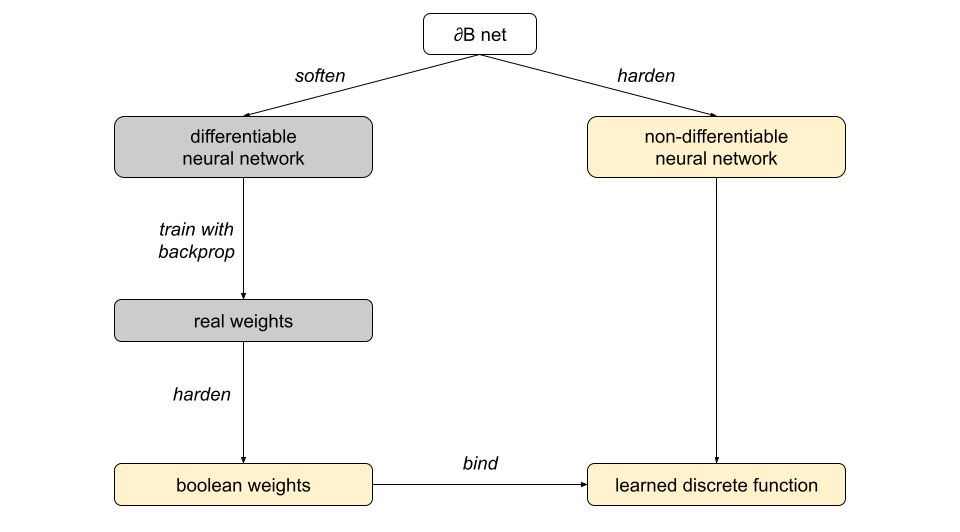
\includegraphics[width=1.0\textwidth]{db-net.png}
	\caption{{\em Learning discrete functions with a $\partial\mathbb{B}$ net.} A $\partial \mathbb{B}$ net specifies (i) a differentiable neural network that is hard-equivalent to (ii) a non-differentiable discrete function. The neural network is trained as normal with backpropagation to yield a set of real weights. The real weights are hardened to boolean values and then bound with the discrete function. The result is a learned discrete function that performs identically to the trained network.}
	\label{fig:main-idea}
\end{figure}

\section{Related work}\label{sec:related-work}

Methods to learn discrete boolean functions can be broadly categorized as either non-differentiable or differentiable.

Non-differentiable approaches include boolean-valued decision trees \citep{BreiFrieStonOlsh84}, random forests \citep{598994}, genetic programming \citep{koza1992genetic} and, more recently, Tsetlin machines \cite{granmo18}. Tsetlin machines represent propositional formulae by collections of simple automata with integer weights optimised by positive and negative feedback defined in terms of a hard threshold function. These models are relatively easier to interpret, compared to deep neural networks, because they directly represent boolean decisions. However, their non-differentiability means it is relatively harder to compose them into larger-scale systems that learn useful representations of high-dimensional data (e.g. NLP, images and audio) without manual feature engineering, although Tsetlin machines show promise on such tasks \citep{Granmo2019TheCT}.

Differentiable approaches include systems that integrate rule-based reasoning with neural components, and binarization techniques that quantize neural networks by converting real-valued weights and activations to binary values. For example, differentiable inductive logic programming \citep{10.5555/3241691.3241692}, neural logic machines \citep{dong2018neural} 
and differentiable neural logic networks \cite{DBLP:phd/basesearch/Payani20} learn first-order logic rules using gradient descent. These systems combine the benefits of logical inference and interpretability with end-to-end differentiability; however, they can require combinatoric enumeration of rulesets and therefore struggle to scale to large datasets. The technique of network binarization aims to significantly reduce model size and inference costs while maintaining predictive accuracy. Binarization reduces a real-valued neural network to a binary network where nonlinear activation functions are replaced by boolean majority functions. For example, BinaryConnect \citep{10.5555/2969442.2969588}, XNOR-Net \citep{10.1007/978-3-319-46493-0_32}, and LUTNet \citep{9026948}, optimize a continuous relaxation or approximation of the binary net during training. However, binary-valued functions are intrinsically non-differentiable and therefore training by gradient descent becomes challenging. Plus, binarization throws away information, which reduces accuracy \citep{QIN2020107281}. 

Clearly, the design-space of algorithms that learn boolean functions is large, with various trade-offs. In this paper we investigate an under-explored area of the design-space where a differentiable neural network is semantically equivalent, without approximation or loss, to an arbitrarily complex boolean function. We aim to combine the benefits of deep neural networks trained by gradient descent with the efficiency, interpretability and logical bias of boolean functions -- but without loss of accuracy.

\section{$\partial\mathbb{B}$ nets}

A $\partial \mathbb{B}$ net has two aspects, a soft net and a hard net. Both nets use bits to represent transitory values and learnable weights. However, a soft net uses soft-bits and a hard net uses hard-bits.

\begin{definition}[Soft-bits and hard-bits]
A {\em soft-bit} is a real value in the range $[0,1]$ and a {\em hard-bit} is a boolean value from the set $\{0,1\}$. A soft-bit, $x$, is {\em high} if $x>1/2$, otherwise it is {\em low}.
\end{definition}

A hardening function converts soft-bits to hard-bits.

\begin{definition}[Hardening]
The {\em hardening} function, $\operatorname{harden}(x_{1}, \dots, x_{n}) = [f(x_{1}), \dots, f(x_{n})]$, converts soft-bits to hard-bits, where
\begin{equation*}
f(x) =
\begin{cases}
1 & \text{if } x > 1/2 \\
0 & \text{otherwise.}
\end{cases}
\end{equation*}
\end{definition}

The soft-bit value $1/2$ is therefore a threshold. Above this threshold the soft-bit represents $\text{True}$, otherwise it represents $\text{False}$.

A soft net is any differentiable function, $f$, that `hardens' to a semantically equivalent discrete function, $g$. For example, if $f(x) = 1 - x$, where $x \in [0,1]$, and $g(y) = \neg y$, where $y \in \{0,1\}$ then: if $x$ is high (resp. low) then both $f(x)$ and $g(\operatorname{harden}(x))$ are low (resp. high). In other words, $f$ is hard-equivalent to boolean negation. More generally:

\begin{definition}[Hard-equivalence]
	A function, $f: [0,1]^n \rightarrow [0,1]^m$, is {\em hard-equivalent} to a discrete function, $g: \{1,0\}^n \rightarrow \{1,0\}^m$,	if
	\begin{equation*}
	\operatorname{harden}(f(\operatorname{harden}({\bf x}))) = g(\operatorname{harden}({\bf x}))
	\end{equation*}
for all ${\bf x} \in [0,1]^{n}$. For shorthand write $f \equiv g$.
\end{definition}

Neural networks are typically composed of nonlinear activation functions (for representational generality) that are strictly monotonic (so gradients always exist that link changes in inputs to outputs) and differentiable (so gradients reliably represent the local loss surface). Activation functions that are monotonic but not strictly so (and therefore some gradients are zero) and differentiable almost everywhere (and therefore some gradients are undefined) also work, e.g. RELU \citep{10.5555/3104322.3104425}. $\partial \mathbb{B}$ nets are arbitrary compositions of `activation' functions that also satisfy these properties but in addition are hard-equivalent to boolean functions (and natural generalisations).

\begin{figure}[t]
	\centering
	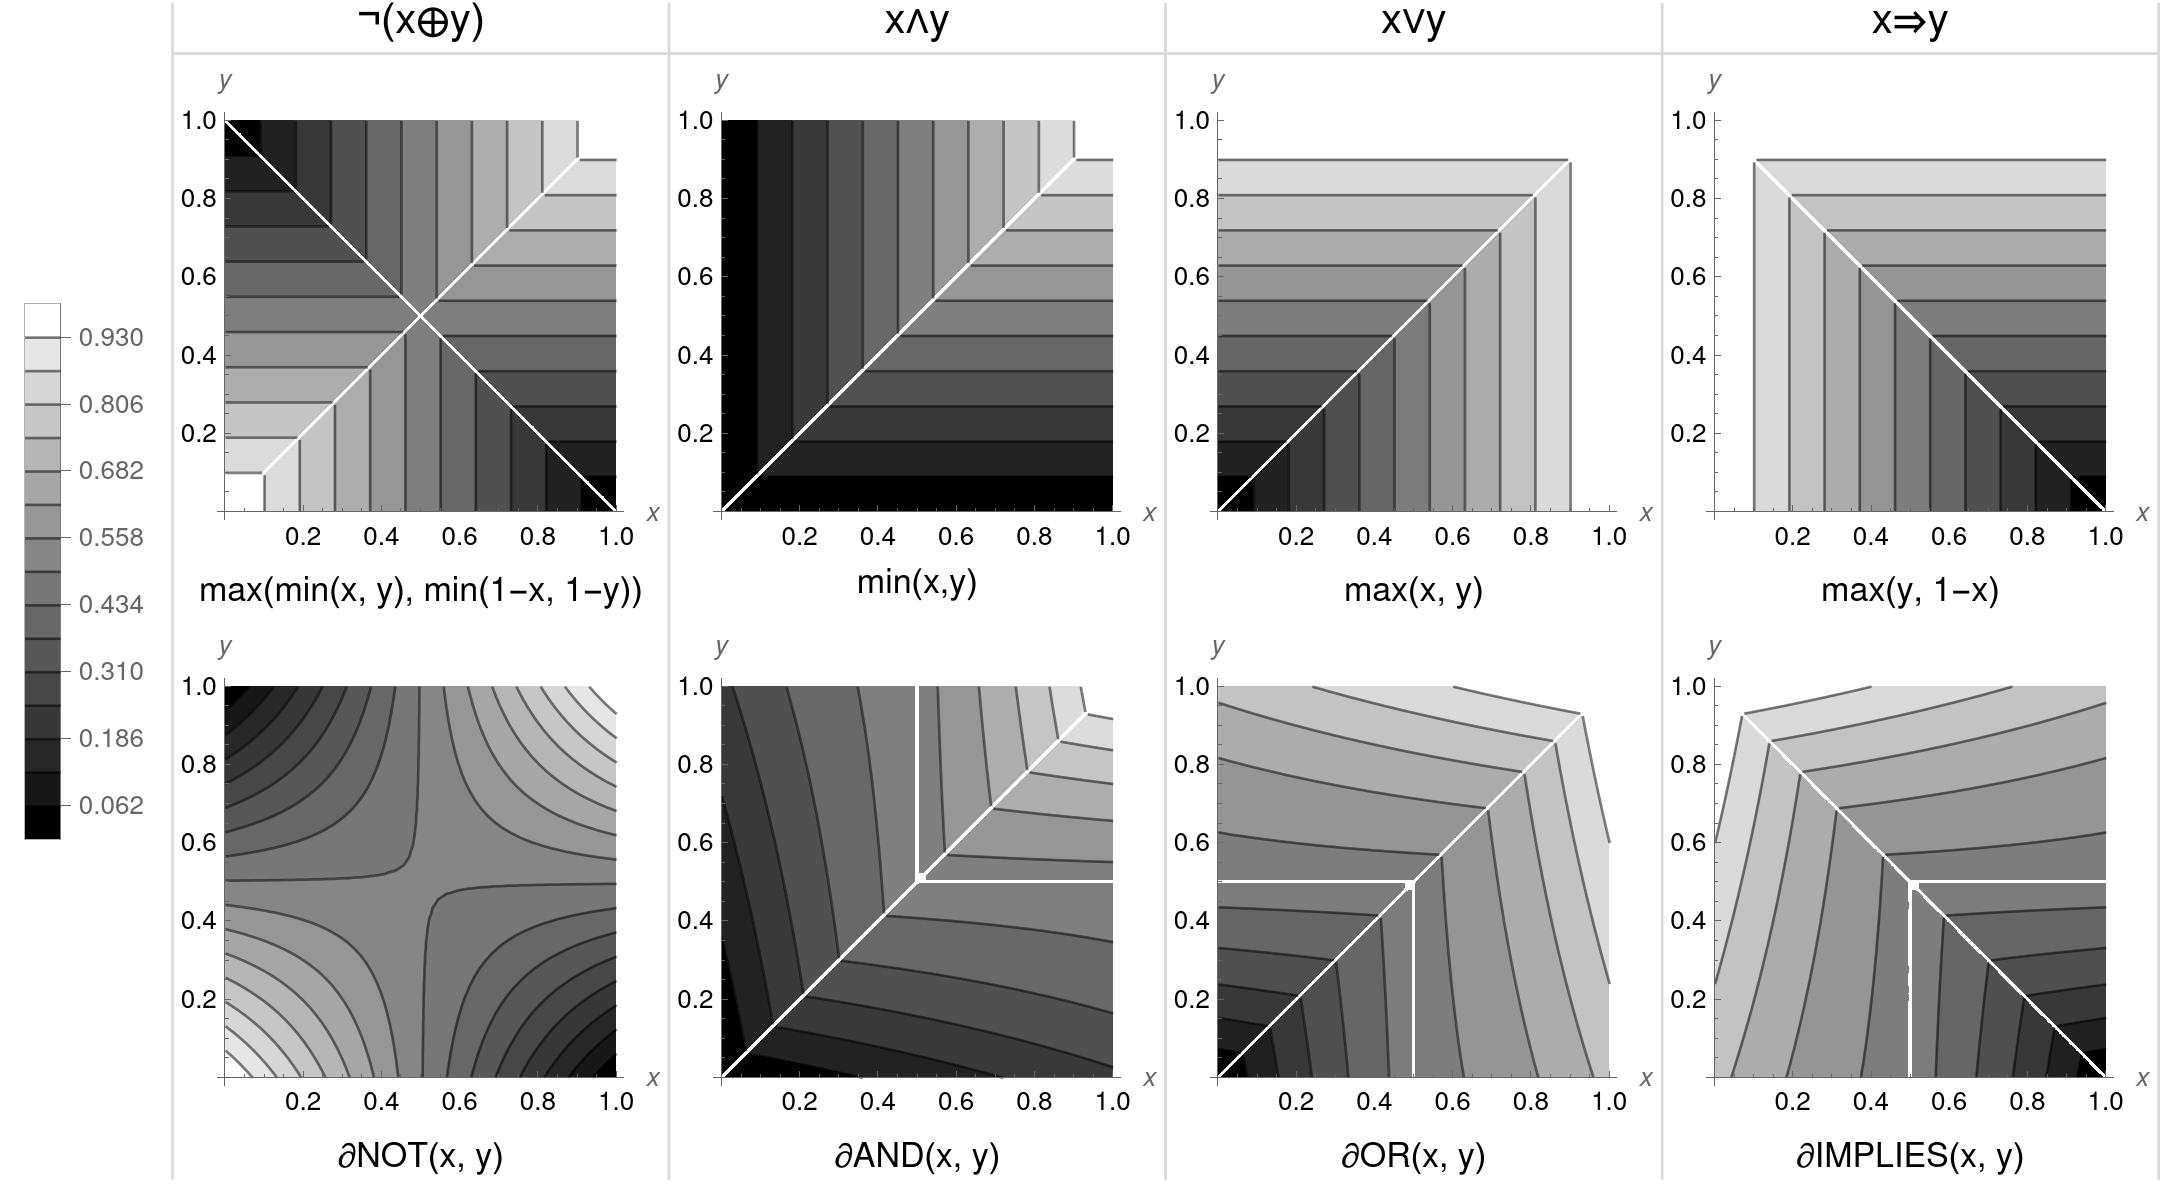
\includegraphics[trim=0pt 0pt 0pt 0pt, clip, width=1.0\textwidth]{logic-gates.png}
	\caption{{\em Gradient-rich versus gradient-sparse differentiable boolean functions.} Each column contains contour plots of functions $f(x,y)$ that are hard-equivalent to a boolean function (one of $\neg(x \oplus y)$, $x \wedge y$, $x \vee y$, or $x \Rightarrow y$). Every function is continuous and differentiable almost everywhere (white lines indicate non-continuous derivatives). The upper plots are gradient-sparse, where vertical and horizontal contours indicate the function is constant with respect to one of its inputs, i.e. $\partial f/\partial y = 0$ or $\partial f/\partial x = 0$. The lower plots are gradient-rich, where the curved contours indicate the function always varies with respect to any of its inputs, i.e. $\partial f/\partial y \neq 0$ and $\partial f/\partial x \neq 0$. $\partial \mathbb{B}$ nets use gradient-rich functions to ensure that error is always backpropagated to all inputs.} 
	\label{fig:gradient-rich}
\end{figure}

\subsection{Learning to negate}

We aim to learn to negate a boolean value, $x$, or simply leave it unaltered. Represent this decision by a boolean weight, $w$, where low $w$ means negate and high $w$ means do nothing. The boolean function that meets this requirement is $\neg(x \oplus w)$. However, this function is not differentiable. We therefore define the differentiable function,
	\begin{equation*}
	\begin{aligned}
	\partial_{\neg}: [0, 1]^{2} &\to [0,1], \\
	(w, x) &\mapsto 1 - w + x (2w - 1)\text{,}
	\end{aligned}
	\end{equation*}
where $\partial_{\neg}(w, x) \equiv \neg(x \oplus w)$ (see proposition \ref{prop:not}).

TODO: See \cite{VANKRIEKEN2022103602} for comparable approaches to activation functions that represent logical operations (Godel, product etc.)

Product logics, where for example $f(x,y) = x y$ is as a soft version of $x \wedge y$, although hard-equivalent at extreme values, e.g. $f(1,1)=1$ and $f(0,1)=0$, are not hard-equivalent at intermediate values, e.g. $f(0.6, 0.6) = 0.36 \not\equiv 1$. G\"{o}del-style $\operatorname{min}$ and $\operatorname{max}$ functions, although hard-equivalent over the entire soft-bit range, i.e. $\operatorname{min}(x,y) \equiv x \wedge y$ and $\operatorname{min}(x,y) \equiv x \vee y$, are gradient-sparse in the sense that their outputs are not always a function of all their inputs, e.g. $\frac{\partial}{\partial x} \operatorname{max}(x,y) = 0$ when $(x,y)=(0.1, 0.9)$. So although the composite function $\operatorname{max}(\operatorname{min}(w, x), \operatorname{min}(1-w, 1-x))$ is differentiable and $\equiv \neg(x \oplus w)$ it does not always backpropagate error to its inputs. In contrast, $\partial_{\neg}$ is a gradient-rich function that always backpropagates error to its inputs (see figure \ref{fig:gradient-rich}). 

\subsection{Margin packing}

Say we aim to construct a differentiable analogue of $x \wedge y$. Note that $\operatorname{min}(x,y)$ essentially selects one of $x$ or $y$ as a representative soft-bit that is guaranteed hard-equivalent to $x \wedge y$. However, by selecting only one of $x$ or $y$ then $\operatorname{min}$ is also guaranteed to be gradient-sparse. We define a `margin packing' method to solve this dilemma.

The main idea of margin packing is (i) select a representative bit that is hard-equivalent to the target discrete function, and then (ii) pack a fraction of the margin between the representative bit and the hard threshold $1/2$ with gradient-rich information. The result is an augmented bit that is a function of all inputs yet hard-equivalent to the target function.

\begin{figure}[t]
	\centering
	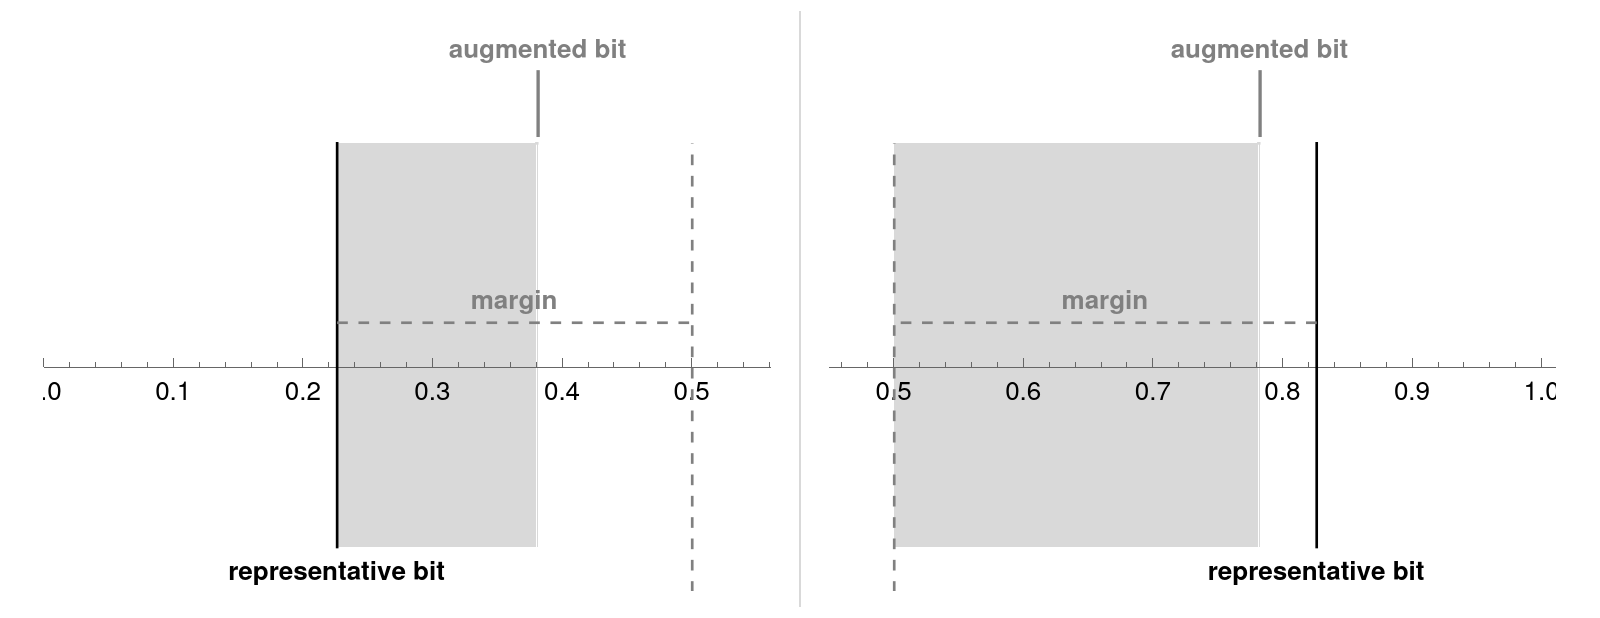
\includegraphics[trim=30pt 5pt 30pt 10pt, clip, width=1.0\textwidth]{margin-trick.png}
	\caption{{\em Margin packing for constructing gradient-rich, hard-equivalent functions}. A representative bit, $z$, is hard-equivalent to a discrete target function but gradient-sparse (e.g. $z=\operatorname{min}(x,y) \equiv x \wedge y$). On the left $z$ is low, $z<1/2$; on the right $z$ is high, $z>1/2$. We can pack a fraction of the margin between $z$ and the hard threshold $1/2$ with additional gradient-rich information without affecting hard-equivalence. A natural choice is the mean soft-bit, $\bar{\bf x} \in [0,1]$. The grey shaded areas denote the packed margins and the final augmented bit. On the left $\approx 60\%$ of the margin is packed; on the right $\approx 90\%$.}
	\label{fig:margin-trick}
\end{figure}
% On the left, ${\bf x}=[0.9,0.23]$, $z=0.23$, $\bar{\bf x}=0.57$ and therefore $\approx 60\%$ of the margin is packed; on the right, ${\bf x}=[0.9,0.83]$,  $z=0.83$, $\bar{\bf x}=0.87$, and therefore $\approx 90\%$ of the margin is packed.

More concretely, say we have a vector of soft-bit inputs ${\bf x}$ and the $i$th element represents the target discrete function (e.g. if our target is $x \wedge y$ then ${\bf x}=[x,y]$ and $i$ is 1 if $x<y$ and $i=2$ otherwise). Now, if we pack only a fraction of the available margin, $|x_{i}-1/2|$, we will not cross the $1/2$ threshold and break the hard-equivalence of the representative bit. The average soft-bit value, $\bar{\bf x} \in [0,1]$, is just such a gradient-rich fraction. We therefore define 
\begin{equation*}
\begin{aligned}
\operatorname{margin-fraction}: [0,1]^{n} \times 1,2,\dots,n &\to [0,1],\\
({\bf x}, i) &\mapsto \bar{\bf x} \times \left|x_{i} - 1/2\right| \text{.}
\end{aligned}
\end{equation*}
The packed fraction, $\bar{\bf x}$, of the margin increases or decreases with the average soft-bit value. The available margin, $\left|x_{i} - 1/2\right|$, tends to zero as the representative bit, $x_{i}$, tends to the hard threshold $1/2$. At the threshold point there is no margin to pack. Now, define the augmented bit as
\begin{equation}
\begin{aligned}
\operatorname{augmented-bit}: [0,1]^{n} \times 1,2,\dots,n &\to [0,1],\\
({\bf x}, i) &\mapsto 
\begin{cases}
1/2 + \operatorname{margin-fraction}({\bf x}, i) & \text{if } x_{i} > 1/2 \\
x_{i} + \operatorname{margin-fraction}({\bf x}, i) & \text{otherwise.}
\end{cases}
\end{aligned}
\label{eq:augmented-bit}
\end{equation}
If the representative bit is high (resp. low) then the augmented bit is also high (resp. low). 
But the augmented bit has a higher (resp. lower) value than the representative bit when below (resp. above) the $1/2$ threshold. The difference depends on the size of the available margin and the mean soft-bit value. Almost everywhere, an increase (resp. decrease) of the mean soft-bit increases (resp. decreases) the value of the augmented bit (see figure \ref{fig:margin-trick}). Note that if the $i$th bit is representative (i.e. hard-equivalent to the target function) then so is the augmented bit (see lemma \ref{prop:augmented}). We use margin packing, where appropriate, to define gradient-rich, hard-equivalents of boolean functions.

\subsection{Differentiable $\wedge$}

We aim to construct a differentiable analogue of the boolean function $\bigwedge_{i=1}^{n} x_i$. A representative bit is $\operatorname{min}(x_{1},\dots,x_{n})$. The function
\begin{equation*}
\begin{aligned}
\partial_{\wedge}: [0,1]^{n} &\to [0,1], \\
{\bf x} &\mapsto \operatorname{augmented-bit}({\bf x}, \operatorname{argmin}\limits_{i} x[i])
\end{aligned}
\end{equation*}
is therefore hard-equivalent to the boolean function $\bigwedge_{i=1}^{n} x_i$ (see proposition \ref{prop:and}). In the special case $n=2$ we get the piecewise function,
\begin{equation*}
\partial_{\wedge}\!(x, y) =
	\begin{cases}
	1/2 + 1/2(x + y)(\operatorname{min}(x,y) - 1/2) & \text{if } \operatorname{min}(x,y) > 1/2 \\
	\operatorname{min}(x,y) + 1/2(x + y)(1/2 - \operatorname{min}(x,y)) & \text{otherwise.}
	\end{cases}
\end{equation*}
Note that $\partial_{\wedge}$ is differentiable almost everywhere and gradient-rich (see figure \ref{fig:gradient-rich}).

\subsection{Differentiable $\vee$}

The differentiable analogue of $\vee$ is identical to $\wedge$, except the representative bit is selected by $\operatorname{max}$. The function
\begin{equation*}
\begin{aligned}
\partial_{\vee}: [0,1]^{n} &\to [0,1], \\
{\bf x} &\mapsto \operatorname{augmented-bit}({\bf x}, \operatorname{argmax}\limits_{i} x[i])
\end{aligned}
\end{equation*}
is hard-equivalent to the boolean function $\bigvee_{i=1}^{n} x_i$ (see proposition \ref{prop:or}). Note that $\partial_{\vee}$ is differentiable almost everywhere and gradient-rich (see figure \ref{fig:gradient-rich}).

\begin{comment}
Define 
\begin{equation*}
\begin{aligned}
\partial_{\vee}\!(x, y) =
\begin{cases}
1/2 + 1/2(x + y)(\operatorname{max}(x,y) - 1/2) & \text{if } \operatorname{max}(x,y) > 1/2 \\
\operatorname{max}(x,y) + 1/2(x + y)(1/2 - \operatorname{max}(x,y)) & \text{otherwise.}
\end{cases}
\end{aligned}
\end{equation*}
\begin{comment}
\begin{equation*}
\begin{aligned}
\partial_{\vee}: [0,1]^{2} &\to [0,1], \\
(x, y) &\mapsto 
\begin{cases}
	1/2 + 1/2(x + y)(m - 1/2) & \text{if } 2m > 1 \\
m + 1/2(x + y)(1/2 - m) & \text{otherwise,}
\end{cases}
\end{aligned}
\end{equation*}
\end{comment}

\subsection{Differentiable $\Rightarrow$}

The differentiable analogue of $\Rightarrow$ is defined in terms of $\partial_{\vee}$. The function
\begin{equation*}
\begin{aligned}
\partial_{\Rightarrow}: [0,1]^{2} &\to [0,1],\\
(x, y) &\mapsto \partial_{\vee}\!(y, 1-x)\text{,}
\end{aligned}
\end{equation*}
is hard-equivalent to $x \Rightarrow y$ (see proposition \ref{prop:implies}). We may define  analogues of all the basic boolean operators in a similar manner.

\subsection{Differentiable majority}

\begin{figure}[t]
	\centering
	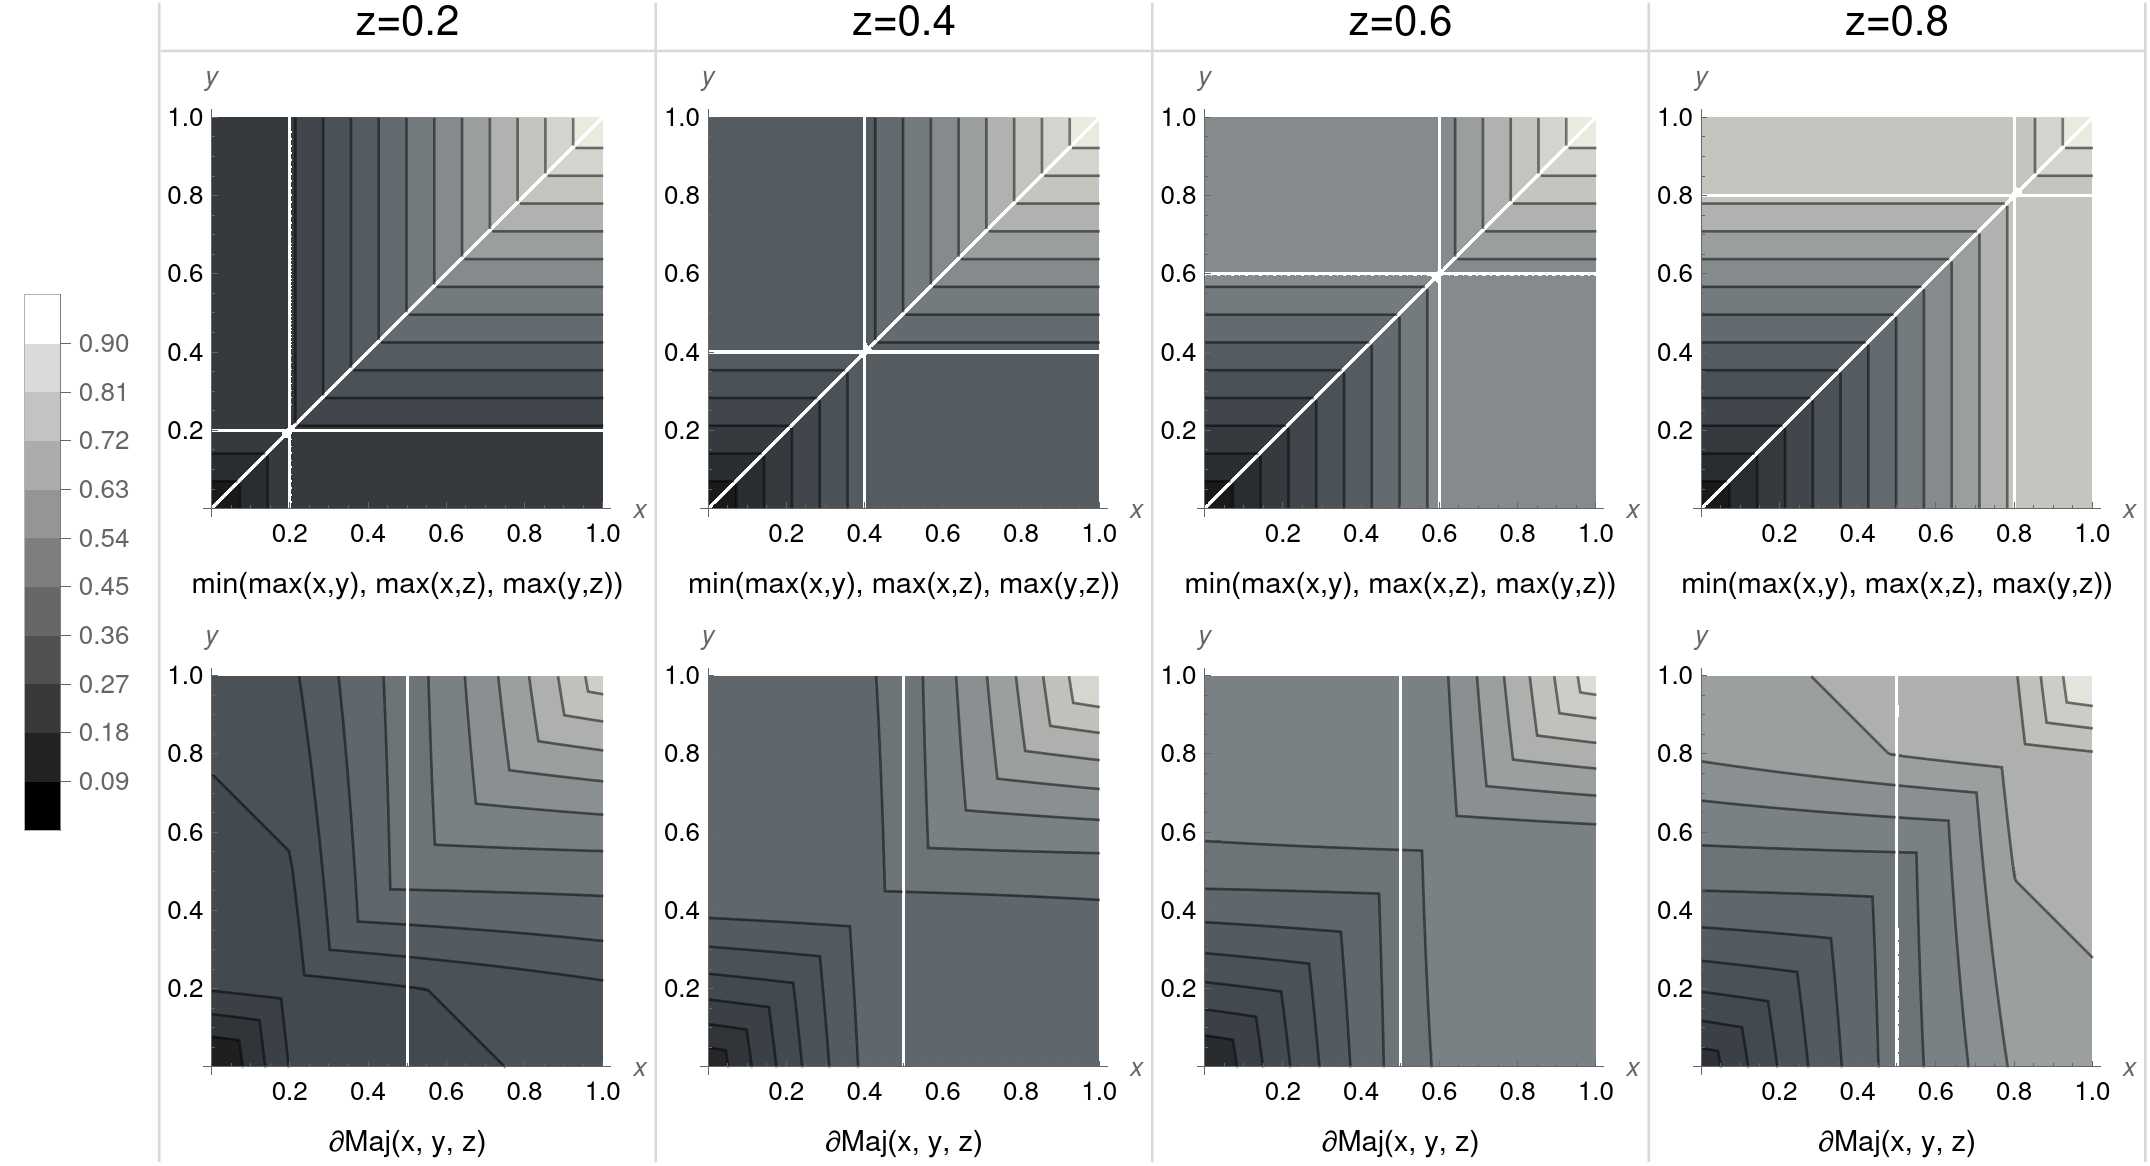
\includegraphics[trim=0pt 0pt 0pt 0pt, clip, width=1.0\textwidth]{majority-gates.png}
	\caption{{\em Differentiable boolean majority.} The boolean majority function for three variables in DNF form is $\operatorname{Maj}(x,y,z) = (x \wedge y) \vee (x \wedge y) \vee (y \wedge z)$. The upper row contains contour plots of $f(x,y,z) = \operatorname{min}(\operatorname{max}(x,y), \operatorname{max}(x,z), \operatorname{max}(y,z))$ for values of $z \in \{0.2, 0.4, 0.6, 0.8\}$. $f$ is differentiable and $\equiv \operatorname{Maj}$ but gradient-sparse (vertical and horizontal contours indicate constancy with respect to an input). Also, the number of terms in $f$ grows exponentially with the number of variables. The lower row contains contour plots of $\partial\!\operatorname{Maj}(x,y,z)$ for the same values of $z$. $\partial\!\operatorname{Maj}$ is differentiable and $\equiv \operatorname{Maj}$ yet gradient-rich (curved contours indicate variability with respect to any inputs). In addition, the number of terms in $\partial\!\operatorname{Maj}$ is constant with respect to the number of variables.} 
	\label{fig:majority-plot}
\end{figure}

The boolean majority function is particularly important for tractable learning because it is a threshold function:
\begin{equation*}
\begin{aligned}
\operatorname{Maj}: \{0,1\}^{n} &\to \{0,1\},\\
{\bf x} &\mapsto \left\lfloor
\frac{1}{2} + \frac{\sum_{i=1}^{n} x_{i} - 1/2}{n}
\right\rfloor\text{,}
\end{aligned}
\end{equation*}
where we count $\operatorname{False}$ as $0$ and $\operatorname{True}$ as $1$. Interpret each input bit $x_{i}$ as a vote, yes or no, for a binary decision. If the majority of voters are in favour then $\operatorname{Maj}$ outputs 1. The majority function, in the context of a predictive model, aggregates multiple bits of weak evidence into a hard decision. Neural network binarization transforms real-valued activation functions into boolean threshold functions \citep{10.5555/3157382.3157557}, which indicates their close association. We aim to construct a differentiable analogue of $\operatorname{Maj}$.

$\operatorname{Maj}$ for $n$ bits in DNF form is a disjunction of $\binom{n}{k}$ conjunctive clauses of size $k$, where $k=\lceil n/2 \rceil$ and each clause checks whether a unique combination of a majority of the $n$ bits are all high; e.g. $\operatorname{Maj}(x, y, z) = (x \wedge y) \vee (x \wedge y) \vee (y \wedge z)$. Therefore, we could in principle implement a differentiable analogue of $\operatorname{Maj}$ in terms of $\partial_{\wedge}$ and $\partial_{\vee}$. However, the number of terms grows exponentially with the number of variables (e.g. $n=50$ generates over 100 trillion clauses, which is infeasible). There is no known general algorithm for finding the minimal representation of $\operatorname{Maj}$ for arbitrary $n$.

Instead, we trade-off time for memory costs. Observe that if the function $\operatorname{sort}({\bf x})$ sorts the elements of ${\bf x}$ in ascending order then the `median' soft-bit is representative. For example, if ${\bf x} = [0.4, 0.9, 0.2]$ then $\operatorname{sort}({\bf x}) = [0.2, 0.4, 0.9]$ and the `median' bit $x_{2}=0.4$ is low, which is hard-equivalent to $\operatorname{Maj}(0, 1, 0) = 0$. Define the index of the `median' bit by
\begin{equation*}
\begin{aligned}
\operatorname{majority-index}: [0, 1]^{n} & \to \mathbb{Z}_{> 0}\\
{\bf x} & \mapsto \left\lceil \frac{|{\bf x}|}{2} \right\rceil
\text{.}
\end{aligned}
\end{equation*}
Then, applying margin packing, define the differentiable function
\begin{equation*}
\begin{aligned}
	\partial\!\operatorname{Maj}: [0,1]^{n} &\to [0,1], \\
	{\bf x} &\mapsto \operatorname{augmented-bit}(\operatorname{sort}({\bf x}), \operatorname{majority-index}({\bf x}))\text{,}
\end{aligned}
\end{equation*}
which is hard-equivalent to $\operatorname{Maj}$ (see theorem \ref{prop:majority}). Note that $\partial\!\operatorname{Maj}$ is differentiable almost everywhere and gradient-rich (see figure \ref{fig:majority-plot}). If $\operatorname{sort}$ is quicksort then the the average time-complexity of $\partial\!\operatorname{Maj}$ is $\mathcal{O}(n\log{}n)$, which makes $\partial\!\operatorname{Maj}$ more expensive than $\partial_{\neg}$, $\partial_{\wedge}$, $\partial_{\vee}$ and $\partial_{\Rightarrow}$ at training time. However, in the hard $\partial\mathbb{B}$ net we efficiently implement $\operatorname{Maj}$ as a discrete program that simply checks if the majority of bits are high.

TODO: compare to \cite{NEURIPS2019_d8c24ca8}

\subsection{Differentiable counting}

A boolean counting function $f({\bf x})$ has the value $1$ if a counting predicate, $c({\bf x})$, holds over its $n$ inputs. For example, $\partial\!\operatorname{Maj}({\bf x})$ is a boolean counting function where $c({\bf x}) := |\{x_{i} : x_{i} = 1 \}| \geq \lceil \frac{n}{2} \rceil$. We aim to construct a differentiable analogue of $\operatorname{count}({\bf x}, k)$ where $c({\bf x}) := |\{x_{i} : x_{i} = 1 \}| = k$ (i.e. `exactly $k$ high'). This is useful for multiclass classification problems where we interpret $k$ as a class prediction.

As before, we use $\operatorname{sort}$ to trade-off time for memory costs. Observe that if the elements of ${\bf x}$ are in ascending order then, if any soft-bits are high, there exists a unique contiguous pair of indices $(i,i+1)$ where $x_{i}$ is low and $x_{i+1}$ is high, where index $i$ is a direct count of the number of soft-bits that are low in ${\bf x}$. In consequence, define
\begin{equation*}
\begin{aligned}
\partial\!\operatorname{count-hot}: [0,1]^{n} &\to [0,1]^{n+1}, \\
{\bf x} &\mapsto \operatorname{low-high}(\operatorname{sort}({\bf x}))\text{,}
\end{aligned}
\end{equation*}
where 
\begin{equation*}
\begin{aligned}
\operatorname{low-high}: [0,1]^{n} &\to [0,1]^{n+1},\\
{\bf x} &\mapsto \left[ \partial_{\wedge}\!(1, x_{1}), \partial_{\wedge}\!(1 - x_{1}, x_{2}), \dots, \partial_{\wedge}\!(1 - x_{n-1}, x_{n}), \partial_{\wedge}\!(1-x_{n}, 1) \right]\text{.}
\end{aligned}
\end{equation*}
$\partial\!\operatorname{count-hot}({\bf x})$ outputs a 1-hot vector where the index of high bit is the number of low bits in ${\bf x}$. For example, $\partial\!\operatorname{count-hot}([0.1, 0.9, 0.2]) = [0.1, 0.2, \bold{0.8}, 0.1]\text{,}$ indicating that 2 bits are low, and $\partial\!\operatorname{count-hot}([0.6, 0.9, 0.7]) = [\bold{0.6}, 0.4, 0.3, 0.1]\text{,}$ indicating that 0 bits are low. Note that $\partial\!\operatorname{count-hot}$ is differentiable, gradient-rich and hard-equivalent to the boolean function
\begin{equation*}
\begin{aligned}
\operatorname{count-hot}: \{0,1\}^{n} &\to \{0,1\}^{n+1}, \\
{\bf x} &\mapsto \left[\operatorname{k-of-n}({\bf x}, 0), \operatorname{k-of-n}({\bf x}, 1), \dots, \operatorname{k-of-n}({\bf x}, n)\right]\text{,}
\end{aligned}
\end{equation*}
where
\begin{equation*}
\operatorname{k-of-n}({\bf x}, k) = \bigvee_{|S|=k} \bigwedge_{i\in S} x_i \bigwedge_{j\notin S} \neg x_j
\end{equation*}
(see proposition \ref{prop:count}). However, in the hard $\partial\mathbb{B}$ net we efficiently implement $\operatorname{count-hot}$ as a discrete program that simply counts the number of low bits. We can construct various kinds of boolean counting functions from $\partial\!\operatorname{count-hot}$. For example, $\partial\!\operatorname{count}({\bf x}, k)$ is straightforwardly $\partial\!\operatorname{count-hot}({\bf x})[k]$ where we can again use margin-packing to ensure that this single soft-bit is gradient-rich.

This set of basic boolean functions is sufficient to learn non-trivial relationships from data. We now turn to constructing $\partial\mathbb{B}$ nets from compositions of these basic functions.

\subsection{Boolean logic layers}

The possible variety of $\partial\mathbb{B}$ net architectures is similar to standard neural networks. Here we merely define some basic layers that are sufficient for classification problems. Other kinds of layers, such as convolutional, or real encoders and decoders for regression problems, will be addressed in a sequel.

A $\partial_{\neg} \!\operatorname{Layer}$ of width $n$ learns to negate up to $n$ different subsets of the elements of its input vector:
\begin{equation*}
\begin{aligned}
\partial_{\neg} \!\operatorname{Layer}: [0,1]^{n \times m} \times [0,1]^{m} &\to [0,1]^{n \times m}, \\
({\bf W}, {\bf x}) &\mapsto 
\begin{bmatrix}
\partial_{\neg}(w_{1,1}, x_{1}) & \dots & \partial_{\neg}(w_{1,m}, x_{m}) \\
\vdots & \ddots & \vdots \\
\partial_{\neg}(w_{n,1}, x_{1}) & \dots & \partial_{\neg}(w_{n,m}, x_{m})
\end{bmatrix}
\end{aligned}
\end{equation*}
where ${\bf x}$ is a soft-bit input vector, ${\bf W}$ is a weight matrix and $n$ is the layer width.

A $\partial_{\wedge}\!\operatorname{Neuron}$ learns to logically $\wedge$ a subset of its input vector:
\begin{equation*}
\begin{aligned}
\partial_{\wedge}\!\operatorname{Neuron}: [0,1]^{n} \times [0,1]^{n} &\to [0,1], \\
({\bf w}, {\bf x}) &\mapsto \min(\partial_{\Rightarrow}\!(w_{1}, x_{1}), \dots, \partial_{\Rightarrow}\!(w_{n}, x_{n}))\text{,}
\end{aligned}
\end{equation*}
where ${\bf w}$ is a weight vector. Each $\partial_{\Rightarrow}(w_{i},x_{i})$ learns to include or exclude $x_{i}$ from the conjunction depending on weight $w_{i}$. For example, if $w_{i}>0.5$ then $x_{i}$ affects the value of the conjunction because $\partial_{\Rightarrow}(w_{i},x_{i})$ passes-through a soft-bit that is high if $x_{i}$ is high, and low otherwise; but if $w_{i} \leq 0.5$ then $x_{i}$ does not affect the conjunction because $\partial_{\Rightarrow}(w_{i},x_{i})$ always passes-through a high soft-bit. A $\partial_{\wedge}\!\operatorname{Layer}$ of width $n$ learns up to $n$ different conjunctions of subsets of its input (of whatever size).

A $\partial_{\vee}\!\operatorname{Neuron}$ is defined similarly:
\begin{equation*}
\begin{aligned}
\partial_{\vee}\!\operatorname{Neuron}: [0,1]^{n} \times [0,1]^{n} &\to [0,1], \\
({\bf w}, {\bf x}) &\mapsto \max(\partial_{\wedge}\!(w_{1}, x_{1}), \dots, \partial_{\wedge}\!(w_{n}, x_{n}))\text{.}
\end{aligned}
\end{equation*}
Each $\partial_{\wedge}(w_{i},x_{i})$ learns to include or exclude $x_{i}$ from the disjunction depending on weight $w_{i}$. For example, if $w_{i}>0.5$ then $x_{i}$ affects the value of the conjunction because $\partial_{\wedge}(w_{i},x_{i})$ passes-through a soft-bit that is high if $x_{i}$ is high, and low otherwise; but if $w_{i} \leq 0.5$ then $x_{i}$ does not affect the conjunction because $\partial_{\Rightarrow}(w_{i},x_{i})$ always passes-through a low soft-bit. A $\partial_{\vee}\!\operatorname{Layer}$ of width $n$ learns up to $n$ different disjunctions of subsets of its input (of whatever size).

We compose $\partial_{\neg}$, $\partial_{\wedge}$ and $\partial_{\vee}$ layers to learn boolean formulae of arbitrary width and depth.

\subsection{Classification layers}

In classification problems the final layer of a neural network is typically interpreted as a vector of real-valued logits, one for each label. The index of the maximum logit indicates the most probable label. However, we cannot interpret the final layer of a $\partial\mathbb{B}$ net as a vector of logits without violating hard-equivalence. Instead, for classification problems, the final layer of a $\partial\mathbb{B}$ net is a 1-hot soft-bit vector, constructed using $\partial\!\operatorname{count-hot}$, where the index of the high bit indicates the predicted label. The hard net then outputs a 1-hot boolean vector with the identical interpretation.

In addition, at training time, loss functions should be a function of hardened bits, otherwise gradient descent may non-optimally traverse trajectories that take no account of the hard threshold at $1/2$. For example, say that an example is correctly classified by a 1-hot vector with high bit $x=0.51$. Updating the net's weights to change this value to $0.51+\epsilon$ won't increase classification accuracy but may prevent updating the weights to correctly classify another example in the training data. For this reason, $\partial\mathbb{B}$ nets have a final `hardening' layer to ensure that loss is a function of hard, not soft, bits:
\begin{equation*}
\begin{aligned}
\partial\!\operatorname{harden}: [0,1]^{n} &\to [0,1]^{n}, \\
{\bf x} &\mapsto \operatorname{harden}({\bf x})\text{.}
\end{aligned}
\end{equation*}
The $\operatorname{harden}$ function is not differentiable and therefore $\partial\!\operatorname{harden}$ uses the straight-through estimator \citep{DBLP:journals/corr/BengioLC13} during backpropagation. However, by restricting the straight-through estimator to the very final layer we avoid compounding gradient estimation errors to deeper parts of the network. $\partial\!\operatorname{harden}$ is hard-equivalent to a $\operatorname{nop}$.

$\partial\mathbb{B}$ nets can re-use many of the techniques deployed in standard neural networks. For example, for improved generalisation, we define a `boolean' analogue of the dropout layer \citep{JMLR:v15:srivastava14a}:
\begin{equation*}
\begin{aligned}
\partial\!\operatorname{dropout}: [0,1]^{n} \times [0,1] &\to [0,1]^{n}, \\
({\bf x}, p) &\mapsto [f(x_{1}, p), \dots, f(x_{n}, p)]\text{,}
\end{aligned}
\end{equation*}
where
\begin{equation*}
f(x, p) = \begin{cases}
1 - x, & \text{with probability } p \\
x, & \text{otherwise.}
\end{cases}
\end{equation*}
At train time $\partial\!\operatorname{dropout}$ randomly negates soft-bit values with probability $p$. At test time, and in the hard net, $\partial\!\operatorname{dropout}$ is a $\operatorname{nop}$.

\section{Implementation}

The $\partial\mathbb{B}$ net library is open-source and available at {\small \url{https://github.com/Z80coder/db-nets}}.

\section{Experiments}

\subsection{Hardening}

\begin{figure}[t!]
	\centering
	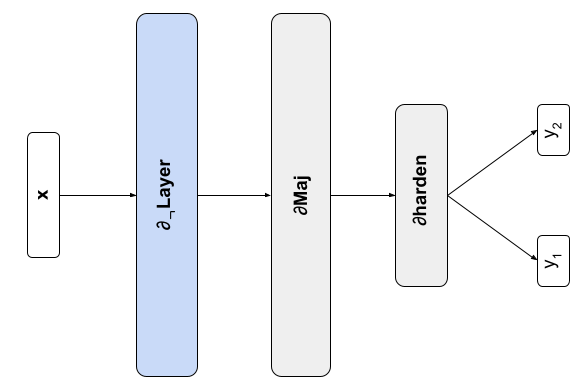
\includegraphics[width=0.65\textwidth]{toy-example-architecture.png}
	\caption{{\em A $\partial\mathbb{B}$ net to illustrate hardening}. The net concatenates a $\partial_{\neg}\!\operatorname{Layer}$ (of width $n$) with a reshaping layer that  outputs two vectors, which get reduced, by a $\partial\!\operatorname{Maj}$ operator,  to 2 soft-bits, one for each class label. A final $\partial\!\operatorname{harden}$ layer ensures the loss is a function of hard bits. When $|{\bf x}|=1$ we choose $n=2$ and therefore the net's weights, once hardened, consume $2$ bits. When $|{\bf x}|=5$ we choose $n=8$ and the weights consume $40$ bits ($5$ bytes).}
	\label{fig:toy-example-architecture}
\end{figure}

We present a toy problem to illustrate hard-equivalence. First, consider the trivial problem of predicting whether a person wears a $\operatorname{t-shirt}$ (label 0) or a $\operatorname{coat}$ (label 1) conditional on the single feature $\operatorname{outside}$ (0 = False, and 1 = True). The training and test data consist of the examples in table \ref{tab:toy1}.

\begin{table}[h!]
	\centering
	\begin{tabular}{|c|c|}
		$\operatorname{outside}$ & $\operatorname{label}$ \\ \hline
		0       & 0     \\
		1       & 1    
	\end{tabular}
	\caption{A trivial learning problem}
	\label{tab:toy1}
\end{table}

We use the $\partial\mathbb{B}$ net described in figure \ref{fig:toy-example-architecture}, which is hard-equivalent to the discrete program:

\begin{lstlisting}[language=Python,style=mystyle,frame=single]
def dbNet(outside):
  return [
    ge(sum((0, not(xor(ne(outside, 0), w1)))), 1),
	ge(sum((0, not(xor(ne(outside, 0), w2)))), 1)
  ]
\end{lstlisting}

with trainable weights $w_{1}$ and $w_{2}$. We randomly initialize the network and train using the RAdam optimizer \citep{Liu2020On} with softmax cross-entropy loss until training and test accuracies are both $100\%$. We harden the learned weights to get $w_{1} = \operatorname{False}$ and $w_{2} = \operatorname{True}$, and bind with the discrete program, which then simplifies to:

\begin{lstlisting}[language=Python,style=mystyle,frame=single]
def dbNet(outside):
	return [not(outside), outside]
\end{lstlisting}

which is directly interpretable as `when outside wear a $\operatorname{coat}$, otherwise wear a $\operatorname{t-shirt}$'.

Hardening scales to arbitrarily complex $\partial\mathbb{B}$ nets, although to interpret the net's predictions more post-training expression simplification is required. Second, we introduce 4 additional boolean features: $\operatorname{very-cold}$, $\operatorname{cold}$, $\operatorname{warm}$, and $\operatorname{very-warm}$. The training and test data consists of examples like those in table \ref{tab:toy2}.

\begin{table}[h!]
	\centering
	\begin{tabular}{|c|c|c|c|c|c|}
		$\operatorname{very-cold}$ & $\operatorname{cold}$ & $\operatorname{warm}$ & $\operatorname{very-warm}$ & $\operatorname{outside}$ & $\operatorname{label}$ \\ \hline
		1 & 0 & 0 & 0 & 0 & 1 \\
		0 & 0 & 0 & 1 & 1 & 1 \\
		0 & 0 & 1 & 0 & 1 & 0 \\
		0 & 0 & 0 & 1 & 0 & 0 \\
		\dots & \dots & \dots & \dots & \dots & \dots
	\end{tabular}
	\caption{A toy learning problem}
	\label{tab:toy2}
\end{table}

We use the same architecture but increase the width of the $\partial_{\neg}\!\operatorname{Layer}$ from 2 to 8. The net is now hard-equivalent to the discrete program:

\begin{comment}
\begin{lstlisting}[language=Python,style=mystyle,frame=single]
def dbNet(very-cold, cold, warm, very-warm, outside):
  return [
    ge(sum((sum((sum((sum((sum((sum((sum((sum((sum((sum((sum((sum((sum((sum((sum((sum((sum((sum((sum((sum((0, not(xor(ne(very-cold, 0), False)))), not(xor(ne(cold, 0), True)))), not(xor(ne(warm, 0), True)))), not(xor(ne(very-warm, 0), True)))), not(xor(ne(outside, 0), True)))), not(xor(ne(very-cold, 0), True)))), not(xor(ne(cold, 0), False)))), not(xor(ne(warm, 0), False)))), not(xor(ne(very-warm, 0), True)))), not(xor(ne(outside, 0), False)))), not(xor(ne(very-cold, 0), False)))), not(xor(ne(cold, 0), False)))), not(xor(ne(warm, 0), True)))), not(xor(ne(very-warm, 0), False)))), not(xor(ne(outside, 0), False)))), not(xor(ne(very-cold, 0), False)))), not(xor(ne(cold, 0), False)))), not(xor(ne(warm, 0), True)))), not(xor(ne(very-warm, 0), False)))), not(xor(ne(outside, 0), False)))), 11),
    ge(sum((sum((sum((sum((sum((sum((sum((sum((sum((sum((sum((sum((sum((sum((sum((sum((sum((sum((sum((sum((0, not(xor(ne(very-cold, 0), True)))), not(xor(ne(cold, 0), False)))), not(xor(ne(warm, 0), False)))), not(xor(ne(very-warm, 0), False)))), not(xor(ne(outside, 0), False)))), not(xor(ne(very-cold, 0), True)))), not(xor(ne(cold, 0), True)))), not(xor(ne(warm, 0), False)))), not(xor(ne(very-warm, 0), True)))), not(xor(ne(outside, 0), True)))), not(xor(ne(very-cold, 0), False)))), not(xor(ne(cold, 0), True)))), not(xor(ne(warm, 0), False)))), not(xor(ne(very-warm, 0), True)))), not(xor(ne(outside, 0), False)))), not(xor(ne(very-cold, 0), False)))), not(xor(ne(cold, 0), True)))), not(xor(ne(warm, 0), False)))), not(xor(ne(very-warm, 0), False)))), not(xor(ne(outside, 0), True)))), 11)]
\end{lstlisting}
\end{comment}

\begin{lstlisting}[language=Python,style=mystyle,frame=single]
def dbNet(very-cold, cold, warm, very-warm, outside):
  return [
    zge(sum((sum((sum((sum((sum((sum((sum((sum((sum((sum((sum((sum((sum((sum((sum((sum((sum((sum((sum((sum((0, not(xor(ne(very-cold, 0), w1)))), not(xor(ne(cold, 0), w2)))), not(xor(ne(warm, 0), w3)))), not(xor(ne(very-warm, 0), w4)))), not(xor(ne(outside, 0), w5)))), not(xor(ne(very-cold, 0), w6)))), not(xor(ne(cold, 0), w7)))), not(xor(ne(warm, 0), w8)))), not(xor(ne(very-warm, 0), w9)))), not(xor(ne(outside, 0), w10)))), not(xor(ne(very-cold, 0), w11)))), not(xor(ne(cold, 0), w12)))), not(xor(ne(warm, 0), w13)))), not(xor(ne(very-warm, 0), w14)))), not(xor(ne(outside, 0), w15)))), not(xor(ne(very-cold, 0), w16)))), not(xor(ne(cold, 0), w17)))), not(xor(ne(warm, 0), w18)))), not(xor(ne(very-warm, 0), w19)))), not(xor(ne(outside, 0), w20)))), 11),
    ge(sum((sum((sum((sum((sum((sum((sum((sum((sum((sum((sum((sum((sum((sum((sum((sum((sum((sum((sum((sum((0, not(xor(ne(very-cold, 0), w21)))), not(xor(ne(cold, 0), w22)))), not(xor(ne(warm, 0), w23)))), not(xor(ne(very-warm, 0), w24)))), not(xor(ne(outside, 0), w25)))), not(xor(ne(very-cold, 0), w26)))), not(xor(ne(cold, 0), w27)))), not(xor(ne(warm, 0), w28)))), not(xor(ne(very-warm, 0), w29)))), not(xor(ne(outside, 0), w30)))), not(xor(ne(very-cold, 0), w31)))), not(xor(ne(cold, 0), w32)))), not(xor(ne(warm, 0), w33)))), not(xor(ne(very-warm, 0), w34)))), not(xor(ne(outside, 0), w35)))), not(xor(ne(very-cold, 0), w36)))), not(xor(ne(cold, 0), w37)))), not(xor(ne(warm, 0), w38)))), not(xor(ne(very-warm, 0), w39)))), not(xor(ne(outside, 0), w40)))), 11)
  ]
\end{lstlisting}
We train the $[w_{1}, \dots, w_{40}]$ soft-bit weights as before then harden to 40 boolean weights and bind with the discrete program. Post-training the program then simplifies to:

\begin{lstlisting}[language=Python,style=mystyle,frame=single]
def dbNet(very-cold, cold, warm, very-warm, outside):
  return [
    4 !very-cold + 4 !cold + (3 warm + !warm) + (very-warm + 3 !very-warm) + (outside + 3 !outside) >= 11,
    (very-cold + 3 !very-cold) + 4 cold + 4 !warm + (3 very-warm + !very-warm) + 2 (outside + !outside) >= 11
  ]
\end{lstlisting}

For example, the label predictions combine multiple pieces of evidence due to the presence of the $\partial\!\operatorname{Maj}$ operator: such as `if not $\operatorname{very-cold}$ and not $\operatorname{cold}$ and not $\operatorname{outside}$ then wear a $\operatorname{t-shirt}$', and `if $\operatorname{cold}$ and not ($\operatorname{warm}$ or $\operatorname{very-warm}$) and $\operatorname{outside}$ then wear a $\operatorname{coat}$' etc.

TODO: note on interpreting and verifying bigger models.

\subsection{Binary Iris}

\begin{figure}[t!]
	\centering
	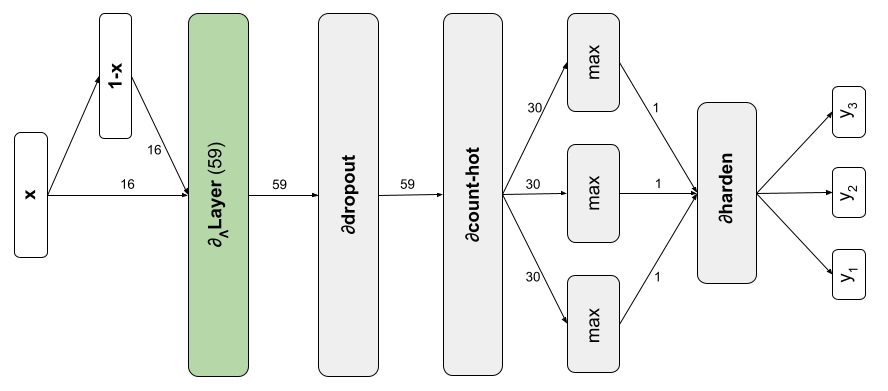
\includegraphics[width=1.0\textwidth]{binary-iris-architecture.png}
	\caption{{\em A $\partial\mathbb{B}$ net for the binary Iris problem}. The net concatenates the soft-bit input, ${\bf x}$ (length 16), with its negation, ${\bf 1 - x}$, and supplies the resulting vector (length 32) to a $\partial_{\wedge}\!\operatorname{Layer}$ (width 59), a $\partial\!\operatorname{dropout}$ layer for improved generalisation, a $\partial\!\operatorname{count-hot}$ layer that generates a 1-hot vector (width 60) that is reduced by $\operatorname{max}$ to a 1-hot vector of 3 classification bits. A final $\partial\!\operatorname{harden}$ ensures the loss is a function of hard bits. The net's weights, once hardened, consume $236$ bytes.}
	\label{fig:binary-iris-architecture}
\end{figure}

The Iris dataset has 150 examples with 4 inputs (sepal length and width, and petal length and width), and 3 labels ({\em setosa}, {\em versicolour}, and {\em virginica}). We use the binary version of the Iris dataset \citep{binary-iris-dataset} where each input float is represented by 4 bits. We perform 1000 experiments, each with a different random seed. Each experiment randomly partitions the data into 80\% training and 20\% test sets. 

We initialize the network, described in figure \ref{fig:binary-iris-architecture}, with all weights $w_{i} = 0.3$ and train for 1000 epochs with the RAdam optimizer and softmax cross-entropy loss. We measure the accuracy of the final net to avoid hand-picking the best configuration. Table \ref{tab:binary-iris-results} compares the $\delta\mathbb{B}$ net against other classifiers  \citep{granmo18}. Naive Bayes performs the worst. The Tsetlin machine performs best on this problem, with the $\partial\mathbb{B}$ net second.

\begin{table}[t]
	\centering
	\begin{tabular}{llllll}
		\cline{2-6}
		\multicolumn{1}{c}{}                       & \multicolumn{5}{c}{\textbf{accuracy}}                                                                                                                                                            \\ \cline{2-6} 
		\multicolumn{1}{l|}{}                      & \multicolumn{1}{l|}{mean}                  & \multicolumn{1}{l|}{5 \%ile}       & \multicolumn{1}{l|}{95 \%ile}       & \multicolumn{1}{l|}{min}           & \multicolumn{1}{l|}{max}            \\ \hline
		\multicolumn{1}{|l|}{Tsetlin}              & \multicolumn{1}{l|}{95.0 +/- 0.2}          & \multicolumn{1}{l|}{86.7}          & \multicolumn{1}{l|}{100.0}          & \multicolumn{1}{l|}{80.0}          & \multicolumn{1}{l|}{100.0}          \\ \hline
		\multicolumn{1}{|l|}{$\partial\mathbb{B}$} & \multicolumn{1}{l|}{\textbf{93.9 +/- 0.1}} & \multicolumn{1}{l|}{\textbf{86.7}} & \multicolumn{1}{l|}{\textbf{100.0}} & \multicolumn{1}{l|}{\textbf{80.0}} & \multicolumn{1}{l|}{\textbf{100.0}} \\ \hline
		\multicolumn{1}{|l|}{neural network}       & \multicolumn{1}{l|}{93.8 +/- 0.2}          & \multicolumn{1}{l|}{86.7}          & \multicolumn{1}{l|}{100.0}           & \multicolumn{1}{l|}{80.0}          & \multicolumn{1}{l|}{100.0}           \\ \hline
		\multicolumn{1}{|l|}{SVM}                  & \multicolumn{1}{l|}{93.6 +/- 0.3}          & \multicolumn{1}{l|}{86.7}          & \multicolumn{1}{l|}{100.0}           & \multicolumn{1}{l|}{76.7}          & \multicolumn{1}{l|}{100.0}           \\ \hline
		\multicolumn{1}{|l|}{naive Bayes}          & \multicolumn{1}{l|}{91.6 +/- 0.3}          & \multicolumn{1}{l|}{83.3}          & \multicolumn{1}{l|}{96.7}           & \multicolumn{1}{l|}{70.0}          & \multicolumn{1}{l|}{100.0}           \\ \hline
	\end{tabular}
	\caption{{\em Ranked binary Iris results}}
	\label{tab:binary-iris-results}
\end{table}


\subsection{Noisy XOR}

\begin{figure}[t!]
	\centering
	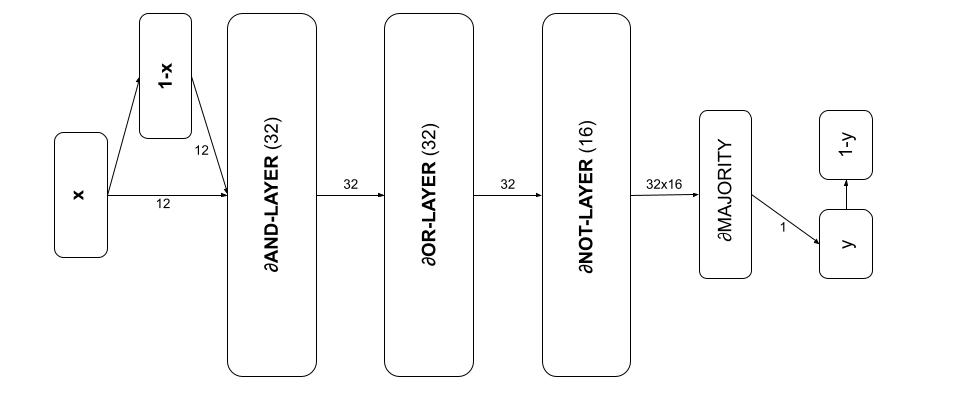
\includegraphics[width=0.95\textwidth]{noisy-xor-architecture.png}
	\caption{{\em A $\partial\mathbb{B}$ net for the noisy xor problem}. The net concatenates the soft-bit input, ${\bf x}$ (length 12), with its negation, ${\bf 1 - x}$, and supplies the resulting vector (length 24) to a $\partial_{\wedge}\!\!\operatorname{Layer}$ (width 32), $\partial_{\vee}\!\!\operatorname{Layer}$ (width 32),  $\partial_{\neg} \!\operatorname{Layer}$ (width 16), and a final $\partial\!\operatorname{Maj}$ to produce a single soft-bit $y \in [0,1]$ (to predict odd parity) and its negation $1-y$ (to predict even parity). The net's weights, once hardened, consume $288$ bytes.}
	\label{fig:noisy-xor-architecture}
\end{figure}

The noisy XOR dataset \citep{noisy-xor-dataset} is an adversarial parity problem with noisy non-informative features. The dataset consists of 10K examples with 12 boolean inputs and a target label (where 0 = odd and 1 = even) that is a XOR function of 2 inputs. The remaining 10 inputs are entirely random. We train on 50\% of the data where, additionally, 40\% of the labels are inverted.

We initialize the network described in figure \ref{fig:noisy-xor-architecture} with random weights distributed close to the hard threshold at $1/2$ (i.e. in the $\partial_{\wedge}\!\operatorname{Layer}$, $w_{i} = 0.501 \times b + 0.3 \times (1-b)$ where $b \sim \operatorname{Bernoulli}(0.01)$; in the $\partial_{\vee}\!\operatorname{Layer}$, $w_{i} = 0.7 \times b + 0.499 \times (1-b)$ where $b \sim \operatorname{Bernoulli}(0.99)$); and in the $\partial_{\neg}\!\operatorname{Layer}$, $w_{i} \sim \operatorname{Uniform}(0.499, 0.501)$. We train for 2000 epochs with the RAdam optimizer and softmax cross-entropy loss. 

We measure the accuracy of the final net on the test data to avoid hand-picking the best configuration. Table \ref{tab:noisy-xor-results} compares the $\partial\mathbb{B}$ net against other classifiers \citep{granmo18}. The high noise causes logistic regression and naive Bayes to randomly guess. The SVM hardly performs better. In constrast, the multilayer neural network, Tsetlin machine, and  $\partial\mathbb{B}$ net all successfully learn the underlying XOR signal. The Tsetlin machine performs best on this problem, with the $\partial\mathbb{B}$ net second.


\begin{table}[t]
	\centering
	\begin{tabular}{llllll}
		\cline{2-6}
		\multicolumn{1}{c}{}                       & \multicolumn{5}{c}{\textbf{accuracy}}                                                                                                                                                            \\ \cline{2-6} 
		\multicolumn{1}{l|}{}                      & \multicolumn{1}{l|}{mean}                  & \multicolumn{1}{l|}{5 \%ile}       & \multicolumn{1}{l|}{95 \%ile}       & \multicolumn{1}{l|}{min}           & \multicolumn{1}{l|}{max}            \\ \hline
		\multicolumn{1}{|l|}{Tsetlin}              & \multicolumn{1}{l|}{99.3 +/- 0.3}          & \multicolumn{1}{l|}{95.9}          & \multicolumn{1}{l|}{100.0}          & \multicolumn{1}{l|}{91.6}          & \multicolumn{1}{l|}{100.0}          \\ \hline
		\multicolumn{1}{|l|}{$\partial\mathbb{B}$} & \multicolumn{1}{l|}{\textbf{97.9 +/- 0.2}} & \multicolumn{1}{l|}{\textbf{95.4}} & \multicolumn{1}{l|}{\textbf{100.0}} & \multicolumn{1}{l|}{\textbf{93.6}} & \multicolumn{1}{l|}{\textbf{100.0}} \\ \hline
		\multicolumn{1}{|l|}{neural network}       & \multicolumn{1}{l|}{95.4 +/- 0.5}          & \multicolumn{1}{l|}{90.1}          & \multicolumn{1}{l|}{98.6}           & \multicolumn{1}{l|}{88.2}          & \multicolumn{1}{l|}{99.9}           \\ \hline
		\multicolumn{1}{|l|}{SVM}                  & \multicolumn{1}{l|}{58.0 +/- 0.3}          & \multicolumn{1}{l|}{56.4}          & \multicolumn{1}{l|}{59.2}           & \multicolumn{1}{l|}{55.4}          & \multicolumn{1}{l|}{66.5}           \\ \hline
		\multicolumn{1}{|l|}{naive Bayes}          & \multicolumn{1}{l|}{49.8 +/- 0.2}          & \multicolumn{1}{l|}{48.3}          & \multicolumn{1}{l|}{51.0}           & \multicolumn{1}{l|}{41.3}          & \multicolumn{1}{l|}{52.7}           \\ \hline
		\multicolumn{1}{|l|}{logistic regression}  & \multicolumn{1}{l|}{49.8 +/- 0.3}          & \multicolumn{1}{l|}{47.8}          & \multicolumn{1}{l|}{51.1}           & \multicolumn{1}{l|}{41.1}          & \multicolumn{1}{l|}{53.1}           \\ \hline
	\end{tabular}
	\caption{{\em Ranked noisy XOR results}}
	\label{tab:noisy-xor-results}
\end{table}


\subsection{MNIST}

TODO

\section{Conclusion}

TODO: we can write boolean functions, soften them, and place them within differentiable neural networks.

\subsubsection*{Acknowledgments}
Thanks to GitHub Next, for sponsoring this research, and Pavel Augustinov, Richard Evans, Johan Rosenkilde, Max Schaefer, Tam\'{a}s Szab\'{o} and Albert Ziegler for helpful discussions and feedback.

\bibliographystyle{iclr2021_conference}
\bibliography{db}

\newpage

\appendix

\section*{Appendix}

\section{Proofs}

\begin{prop}\label{prop:not}
	$\partial_{\neg}(x,y) \equiv \neg (x \oplus y)$.
\begin{proof}
	Table \ref{not-table} is the truth table of the boolean function $\neg (x \oplus w)$, where $h(x) = \operatorname{harden}(x)$.
	\begin{table}[t!]
		\begin{center}
			\begin{tabular}{cccccc}
				\multicolumn{1}{c}{$x$}  &\multicolumn{1}{c}{$y$}  &\multicolumn{1}{c}{$h(x)$}  &\multicolumn{1}{c}{$h(y)$} &\multicolumn{1}{c}{$\partial_{\neg}(h(x), h(y))$} &\multicolumn{1}{c}{$h(\partial_{\neg}(h(x), h(y)))$}
				\\ \hline \\
				$\left[0, \frac{1}{2}\right]$ & $\left[0, \frac{1}{2}\right]$ & 0 & 0 & 1 & 1\\[0.1cm]
				$\left(\frac{1}{2}, 1\right]$ & $\left[0, \frac{1}{2}\right]$ &1 & 0 & 0 & 0\\[0.1cm]
				$\left[0, \frac{1}{2}\right]$ & $\left(\frac{1}{2}, 1\right]$ &0 & 1 & 0 & 0\\[0.1cm]
				$\left(\frac{1}{2}, 1\right]$ & $\left(\frac{1}{2}, 1\right]$ &1 & 1 & 1 & 1\\[0.1cm]
			\end{tabular}
		\end{center}
		\caption{$\partial_{\neg}(x,y) \equiv \neg (y \oplus x)$.}\label{not-table}
	\end{table}
\end{proof}
\end{prop}

\begin{lemma}\label{prop:augmented}
	If a representative bit, $x_{i}$, is hard-equivalent to a target function, $g$, then so is the augmented bit, $z$.
	\begin{proof}
		As $x_{i}$ is representative then $\operatorname{harden}(x_{i}) = g(\operatorname{harden}({\bf x}))$. The augmented bit, $z$, is given by  \eqref{eq:augmented-bit}:
		\begin{equation*}
		z = \begin{cases}
		1/2 + \bar{\bf x}\times|x_{i} - 1/2| & \text{if } x_{i} > 1/2 \\
		x_{i} + \bar{\bf x}\times|x_{i} - 1/2| & \text{otherwise.}
		\end{cases}
		\end{equation*}
		In consequence,
		\begin{equation*}
		\operatorname{harden}(z) = \begin{cases}
		1 & \text{if } x > 1/2 \\
		0 & \text{otherwise,}
		\end{cases}
		\end{equation*}
		since $x_{i} > 1/2 \Rightarrow z > 1/2$ and $x_{i} \leq 1/2 \Rightarrow z \leq 1/2$. Hence, $\operatorname{harden}(z) = \operatorname{harden}(x_{i}) = g(\operatorname{harden}({\bf x}))$
	\end{proof}
\end{lemma}


\begin{prop}\label{prop:and}
	$\partial_{\wedge}\!(x,y) \equiv x \wedge y$.
\begin{proof}
	Table \ref{and-table} is the truth table of the boolean function $x \wedge y$, where $h(x) = \operatorname{harden}(x)$..
	\begin{table}[t!]
		\begin{center}
			\begin{tabular}{cccccc}
				\multicolumn{1}{c}{$x$}  &\multicolumn{1}{c}{$y$}  &\multicolumn{1}{c}{$h(x)$}  &\multicolumn{1}{c}{$h(y)$} &\multicolumn{1}{c}{$\partial_{\wedge}(h(x), h(y))$} &\multicolumn{1}{c}{$h(\partial_{\wedge}(h(x), h(y)))$}
				\\ \hline \\
				$\left[0, \frac{1}{2}\right]$ & $\left[0, \frac{1}{2}\right]$ & 0 & 0 & 0 & 0\\[0.1cm]
				$\left(\frac{1}{2}, 1\right]$ & $\left[0, \frac{1}{2}\right]$ &1 & 0 & $\frac{1}{4}$ & 0\\[0.1cm]
				$\left[0, \frac{1}{2}\right]$ & $\left(\frac{1}{2}, 1\right]$ &0 & 1 & $\frac{1}{4}$ & 0\\[0.1cm]
				$\left(\frac{1}{2}, 1\right]$ & $\left(\frac{1}{2}, 1\right]$ &1 & 1 & 1 & 1\\[0.1cm]
			\end{tabular}
		\end{center}
		\caption{$\partial_{\wedge}(x,y) \equiv x \wedge y$.}\label{and-table}
	\end{table}			
\end{proof}
\end{prop}

\begin{prop}\label{prop:or}
	$\partial_{\vee}\!(x,y) \equiv x \vee y$.
\begin{proof}
	Table \ref{or-table} is the truth table of the boolean function $x \vee y$, where $h(x) = \operatorname{harden}(x)$..
	\begin{table}[t!]
	\begin{center}
		\begin{tabular}{cccccc}
			\multicolumn{1}{c}{$x$}  &\multicolumn{1}{c}{$y$}  &\multicolumn{1}{c}{$h(x)$}  &\multicolumn{1}{c}{$h(y)$} &\multicolumn{1}{c}{$\partial_{\vee}(h(x), h(y))$} &\multicolumn{1}{c}{$h(\partial_{\vee}(h(x), h(y)))$}
			\\ \hline \\
			$\left[0, \frac{1}{2}\right]$ & $\left[0, \frac{1}{2}\right]$ & 0 & 0 & 0 & 0\\[0.1cm]
			$\left(\frac{1}{2}, 1\right]$ & $\left[0, \frac{1}{2}\right]$ &1 & 0 & $\frac{3}{4}$ & 1\\[0.1cm]
			$\left[0, \frac{1}{2}\right]$ & $\left(\frac{1}{2}, 1\right]$ &0 & 1 & $\frac{3}{4}$ & 1\\[0.1cm]
			$\left(\frac{1}{2}, 1\right]$ & $\left(\frac{1}{2}, 1\right]$ &1 & 1 & 1 & 1\\[0.1cm]
		\end{tabular}
	\end{center}
	\caption{$\partial_{\vee}(x,y) \equiv x \vee y$.}\label{or-table}
	\end{table}			
\end{proof}
\end{prop}

\begin{prop}\label{prop:implies}
	$\partial_{\Rightarrow}\!(x,y) \equiv x \Rightarrow y$.
\begin{proof}
	Table \ref{implies-table} is the truth table of the boolean function $x \Rightarrow y$, where $h(x) = \operatorname{harden}(x)$..
	\begin{table}[t!]
	\begin{center}
		\begin{tabular}{cccccc}
			\multicolumn{1}{c}{$x$}  &\multicolumn{1}{c}{$y$}  &\multicolumn{1}{c}{$h(x)$}  &\multicolumn{1}{c}{$h(y)$} &\multicolumn{1}{c}{$\partial \Rightarrow(h(x), h(y))$} &\multicolumn{1}{c}{$h(\partial \Rightarrow(h(x), h(y)))$}
			\\ \hline \\
			$\left[0, \frac{1}{2}\right]$ & $\left[0, \frac{1}{2}\right]$ & 0 & 0 & $\frac{3}{4}$ & 1\\[0.1cm]
			$\left(\frac{1}{2}, 1\right]$ & $\left[0, \frac{1}{2}\right]$ &1 & 0 & 0 & 0\\[0.1cm]
			$\left[0, \frac{1}{2}\right]$ & $\left(\frac{1}{2}, 1\right]$ &0 & 1 & 1 & 1\\[0.1cm]
			$\left(\frac{1}{2}, 1\right]$ & $\left(\frac{1}{2}, 1\right]$ &1 & 1 & $\frac{3}{4}$ & 1\\[0.1cm]
		\end{tabular}
	\end{center}
	\caption{$\partial \Rightarrow(x,y) \equiv x \Rightarrow y$.}\label{implies-table}
	\end{table}			
\end{proof}
\end{prop}

\begin{lemma}
\label{lem:maj}
Let $i$ = $\operatorname{majority-index}({\bf x})$, then the $i$th element of $\operatorname{sort}({\bf x})$ is hard-equivalent to boolean majority, i.e. $\operatorname{harden}(\operatorname{sort}({\bf x})[i]) = \operatorname{Maj}(\operatorname{harden}({\bf x}))$.
\begin{proof}
Let $h$ denote the number of bits that are high in ${\bf x} = [x_{1}, \dots, x_{n}]$. Then indices $\{j : n-h+1 \leq j \leq n\}$ are high in $\operatorname{sort}({\bf x})$. If the majority of bits are high, $h \geq \lfloor n/2 + 1 \rfloor$, then index $j=n - \lfloor n/2 + 1 \rfloor + 1 = n - \lfloor n/2 \rfloor = \lceil n/2 \rceil$ is high in $\operatorname{sort}({\bf x})$. $\operatorname{majority-index}$ selects index $i = \lceil n/2 \rceil$ and therefore $i=j$. Hence, if the majority of bits are high then $\operatorname{sort}({\bf x})[i]$ is high. Similarly, if the majority of bits are low, $h < \lfloor n/2 + 1 \rfloor$, then index $j=n - \lfloor n/2 + 1 \rfloor + 1 = n - \lfloor n/2 \rfloor = \lceil n/2 \rceil$ is low in $\operatorname{sort}({\bf x})$. Hence, if the majority of bits are low then $\operatorname{sort}({\bf x})[i]$ is low.

Note that $h \geq \lfloor n/2 + 1 \rfloor$ implies that $\operatorname{Maj}(\operatorname{harden}({\bf x})) \geq \left\lfloor \frac{1}{2} + \frac{1}{n}\left(\frac{n}{2} + 1 - \frac{1}{2} \right) \right\rfloor \geq \left\lfloor 1 + \frac{1}{2n} \right\rfloor = 1$, and $h < \lfloor n/2 + 1 \rfloor$ implies that $\operatorname{Maj}(\operatorname{harden}({\bf x})) < \left\lfloor 1 + \frac{1}{2n} \right\rfloor = 0$.

In consequence, $\operatorname{harden}(\operatorname{sort}({\bf x})[i]) = \operatorname{Maj}(\operatorname{harden}({\bf x}))$ for all $h \in [0,\dots, n]$.
\end{proof}
\end{lemma}

\begin{theorem}\label{prop:majority}
	$\partial\!\operatorname{Maj} \equiv \operatorname{Maj}$.
\begin{proof}
	$\partial\!\operatorname{Maj}$ augments the representative bit $x_{i} = \operatorname{sort}({\bf x})[\operatorname{majority-index}({\bf x})]$. By lemma \ref{lem:maj}, the representative bit is $\equiv \operatorname{Maj}(\operatorname{harden}({\bf x}))$.
    By lemma \ref{prop:augmented}, the augmented bit, $\operatorname{augmented-bit}(\operatorname{sort}({\bf x}), \operatorname{majority-index}({\bf x}))$, is also $\equiv \operatorname{Maj}(\operatorname{harden}({\bf x}))$. Hence $\partial\!\operatorname{Maj} \equiv \operatorname{Maj}$.
\end{proof}
\end{theorem}

\begin{prop}\label{prop:count}
	$\partial\!\operatorname{count-hot} \equiv \operatorname{count-hot}$.
	\begin{proof}
	Let $l$ denote the number of bits that are low in ${\bf x} = [x_{1},\dots,x_{n}]$, and let ${\bf y} = \partial\!\operatorname{count-hot}({\bf x})$. Then ${\bf y}[l+1]$ is high and any ${\bf y}[i]$, where $i \neq l+1$, is low. Let ${\bf z} = \operatorname{count-hot}(\operatorname{harden}({\bf x}))$. Then ${\bf z}[l+1]$ is high and any ${\bf z}[i]$, where $i \neq l+1$, is low. Hence, $\operatorname{harden}({\bf y}) = {\bf z}$, and therefore $\partial\!\operatorname{count-hot} \equiv \operatorname{count-hot}$.
	\end{proof}
\end{prop}


\end{document}

\begin{comment}
Define
\begin{equation*}
\begin{aligned}
\partial\text{AND-LAYER}: [0,1]^{n \times m} \times [0,1]^{m} &\to [0,1]^{n}, \\
({\bf W}, {\bf x}) &\mapsto [\partial_{\wedge}\operatorname{Neuron}({\bf W}_{1}, {\bf x}), \dots, \partial_{\wedge}\operatorname{Neuron}({\bf W}_{n}, {\bf x})]
\end{aligned}
\end{equation*}
\end{comment}
